\documentclass[12pt, twoside]{book}

% variable values
\input variables.tex

\ifshowframe{}
    \usepackage[a4paper,top=2.5cm,bottom=2.5cm,left=3.5cm,right=2cm,showframe]{geometry}
\else
    \usepackage[a4paper,top=2.5cm,bottom=2.5cm,left=3.5cm,right=2cm]{geometry}
\fi
\usepackage{microtype}
\usepackage[slovak,USenglish]{babel}
\usepackage[utf8]{inputenc}
\usepackage[T1]{fontenc}

\linespread{1.25} % this means 1.5 line spacing

% more package imports and custom commands
\input definitions.tex

\tikzset{every node/.style={circle, draw, fill=black}}

\begin{document}

\ifenglish{}
    \selectlanguage{USenglish}
\else
    \selectlanguage{slovak}
\fi

\frontmatter
\pagenumbering{gobble}

% COVER
\thispagestyle{empty}

{
    \sc\large

    \begin{center}
        \thesisuniversity{}\\
        \thesisfaculty{}

        \vfill

        {\LARGE\thesisname}\\
        \thesistype{}
    \end{center}

    \vfill

    \noindent
    \thesisyear{}\\
    \thesisauthor{}
}

\cleardoublepage{}

% TITLE PAGE
\frontmatter
\thispagestyle{empty}

\begin{center}
    \sc\large
    \thesisuniversity{}\\
    \thesisfaculty{}

    \vfill

    {\LARGE\thesisname}\\
    \thesistype{}
\end{center}

\vfill

\noindent
\begin{tabular}{ll}
    \ifenglish{}Study Programme:\else{}Študijný program:   \fi & \thesisprogramme{}\\
    \ifenglish{}Field of Study: \else{}Študijný odbor:     \fi & \thesisfield{}\\
    \ifenglish{}Department:     \else{}Školiace pracovisko:\fi & \thesisdepartment{}\\
    \ifenglish{}Supervisor:     \else{}Školiteľ:           \fi & \thesissupervisor{}\\
    \ifconsultant{}\ifenglish{}Consultant:\else{}Konzultant:\fi & \thesisconsultant{}\\ \fi
\end{tabular}

\vfill

\noindent
\thesislocation, \thesisyear{}\\
\thesisauthor{}

\cleardoublepage{}

% ASSIGNMENT
\newpage
\thispagestyle{empty}

\noindent
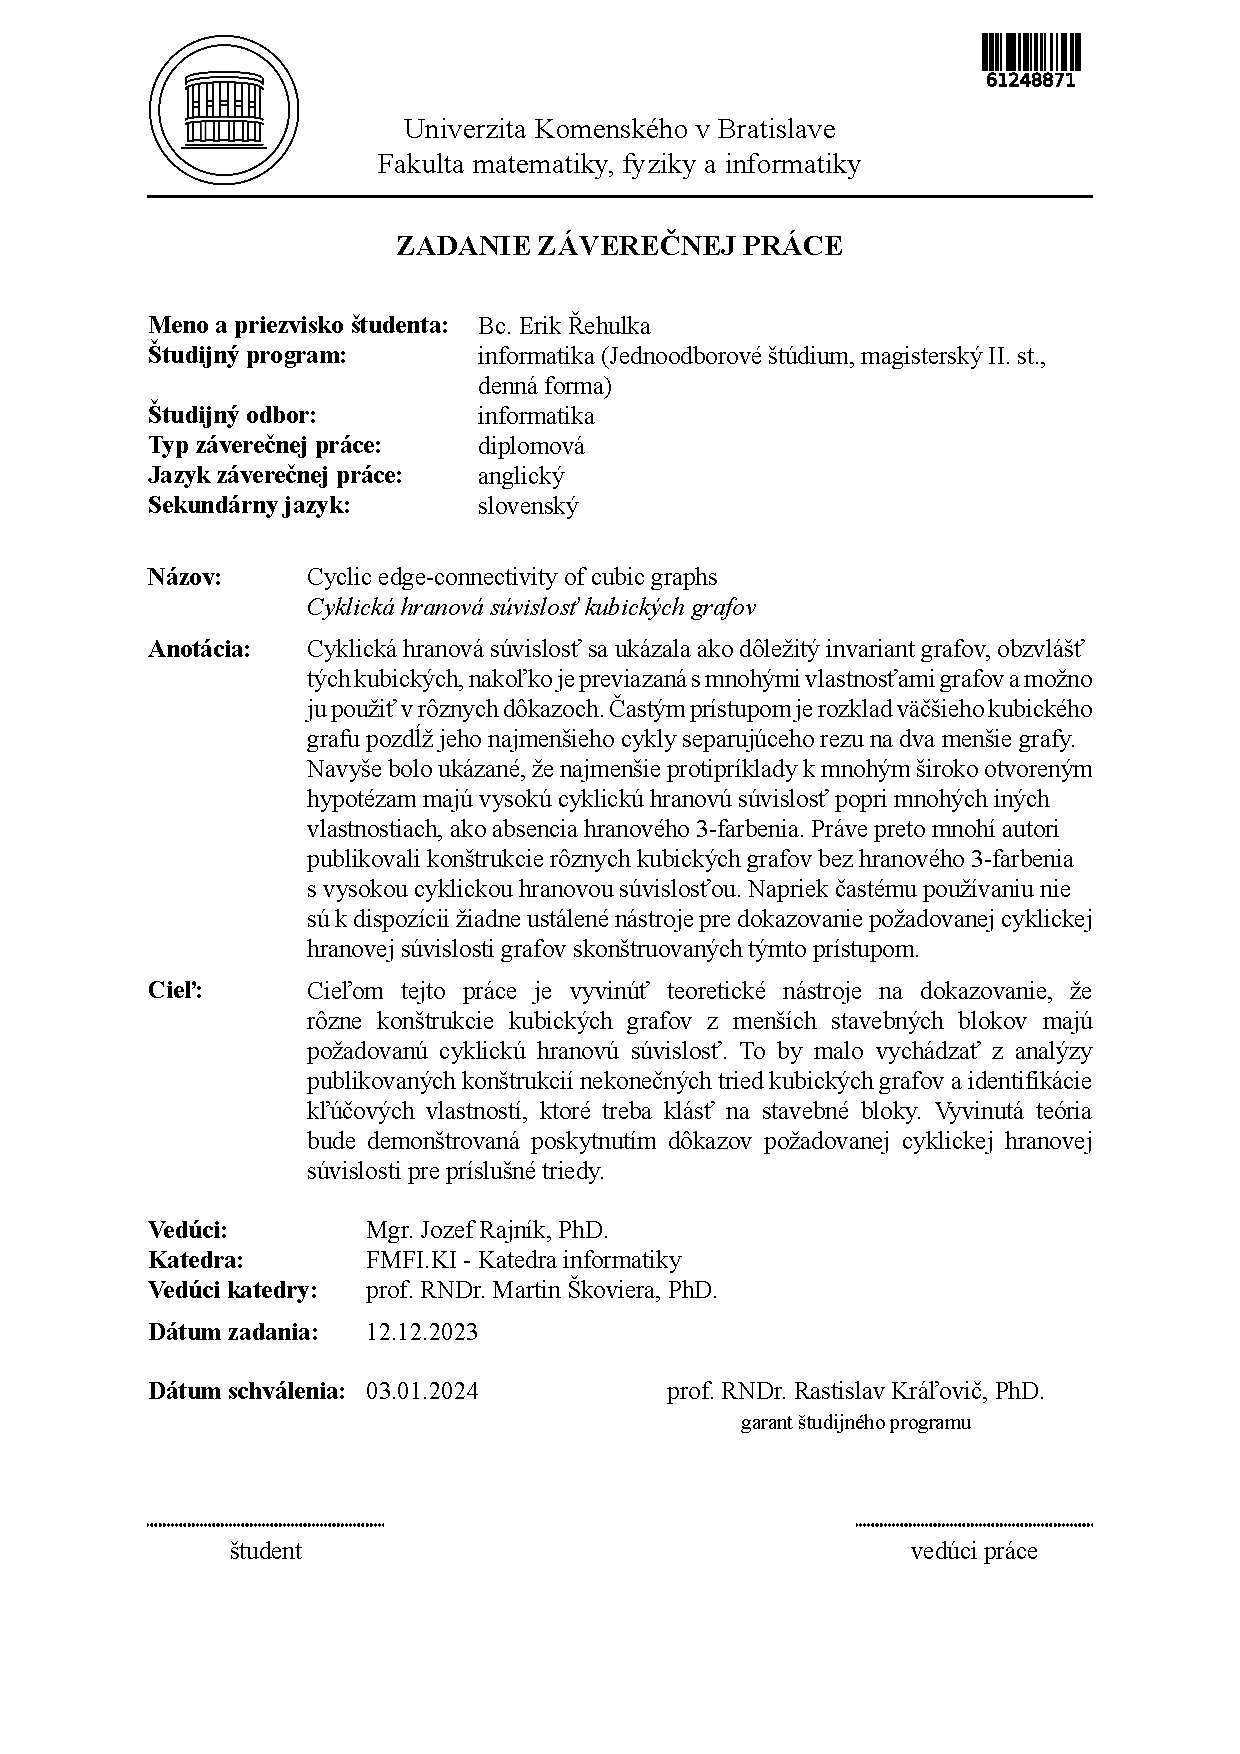
\includegraphics[trim=2.5cm 5cm 2.5cm 0,width=\textwidth]{images/assignment-sk.pdf}

\ifenglish{}
    \newpage
    \thispagestyle{empty}

    \noindent
    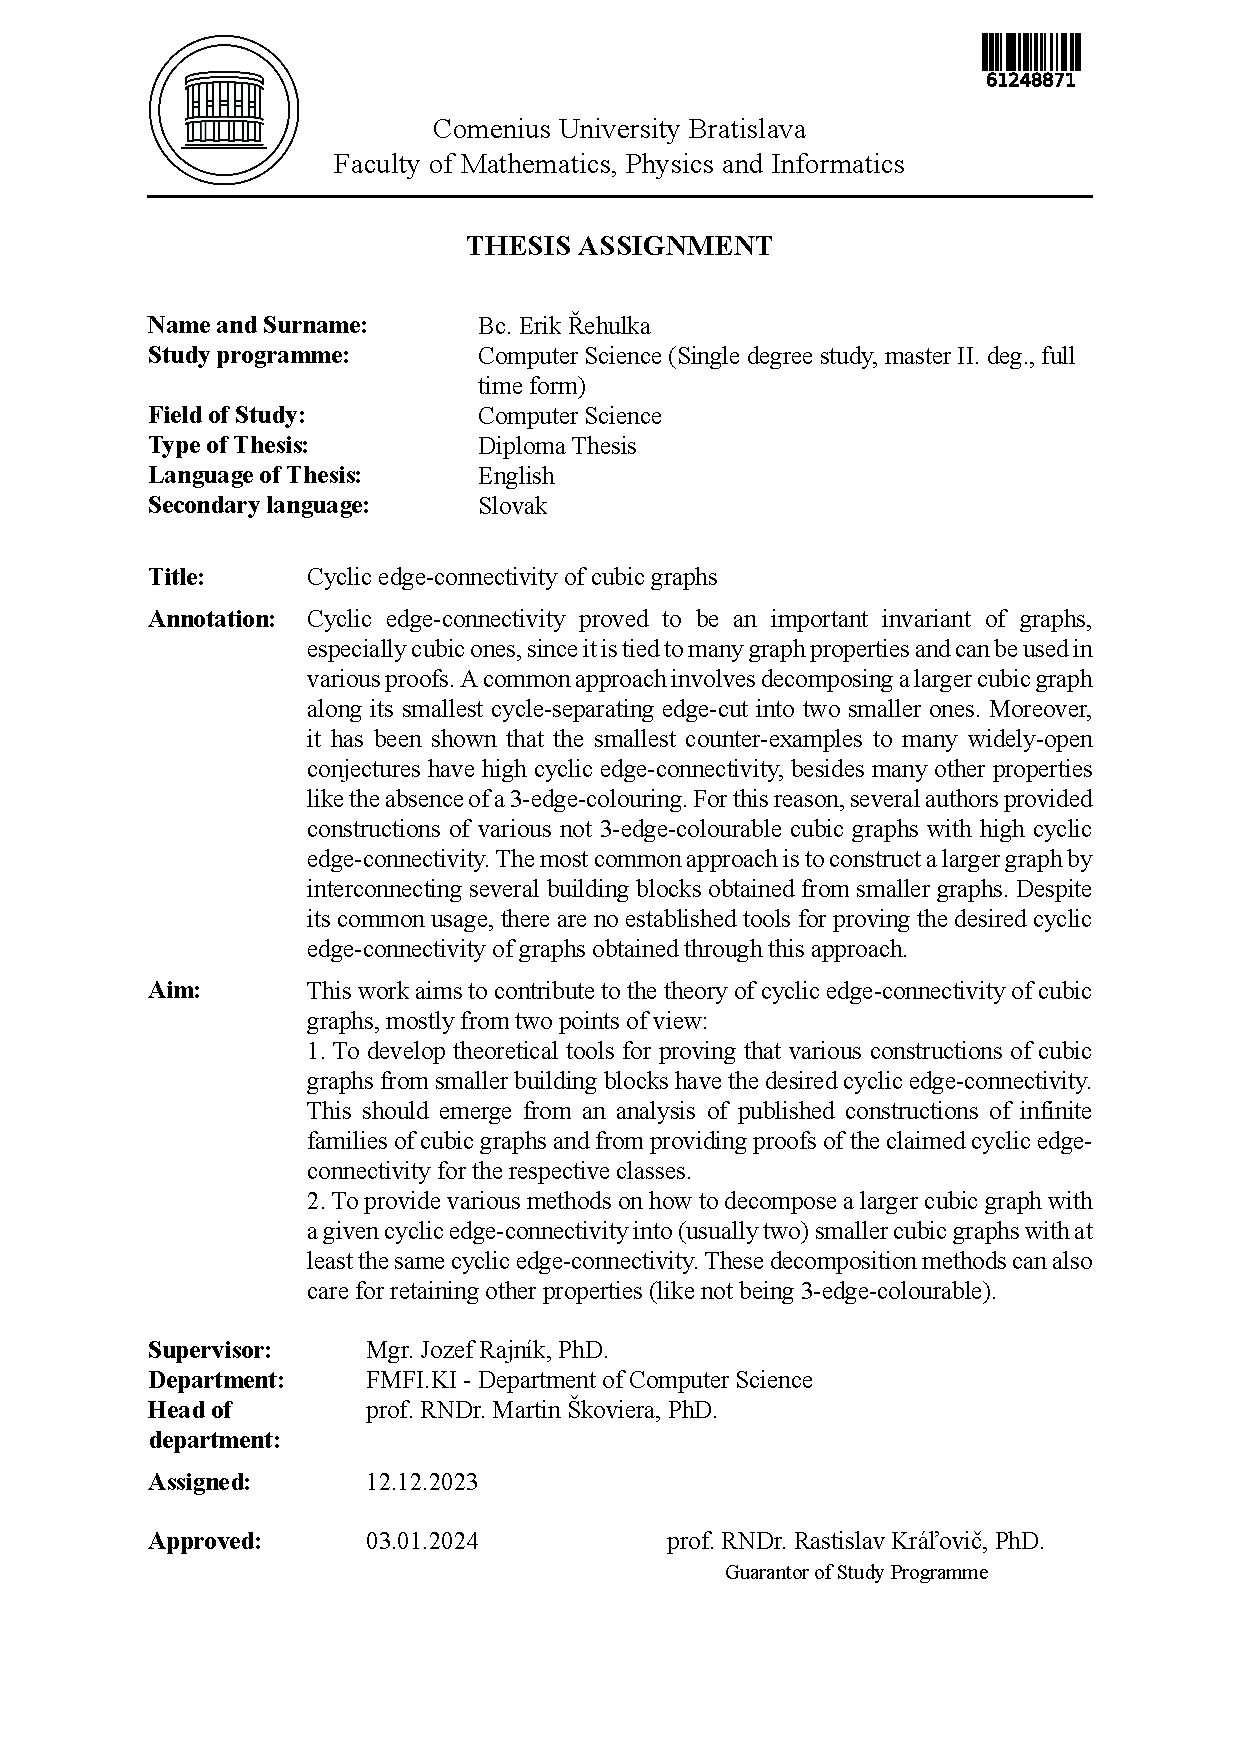
\includegraphics[trim=2.5cm 5cm 2.5cm 0,width=\textwidth]{images/assignment-en.pdf}
\fi

% ACKNOWLEDGEMENTS
\newpage

~\vfill
\paragraph*{\ifenglish{}Acknowledgments:\else{}Poďakovanie:\fi} \thesisacknowledgments{}

% ABSTRACT SK
\newpage

\begin{otherlanguage}{slovak}
    \section*{Abstrakt}

    \thesisabstractsk{}

    \paragraph*{Kľúčové slová:} \thesiskeywordssk{}
\end{otherlanguage}

% ABSTRACT EN
\newpage

\begin{otherlanguage}{USenglish}
    \section*{Abstract}

    \thesisabstracten{}

    \paragraph*{Keywords:} \thesiskeywordsen{}
\end{otherlanguage}

% TABLE OF CONTENTS, LIST OF FIGURES
\newpage
\tableofcontents

\newpage
\listoffigures

% CONTENTS
\mainmatter{}

\chapter*{Introduction}
\addcontentsline{toc}{chapter}{Introduction}
\markboth{Introduction}{Introduction}

In the study of cubic, that is 3-regular graphs, the traditional edge-connectivity faces a natural limitation: it cannot exceed three, the minimum degree of such graphs. This constraint significantly restricts the exploration of properties of cubic graphs with different values of edge-connectivity.

Cyclic edge-connectivity, on the other hand, offers a wider range of values by imposing additional condition on edge-cuts. Specifically, the cyclic edge-connectivity of a graph $G$ is defined as the size of the smallest cycle-separating edge-cut -- an edge-cut whose removal yields two components, each containing a cycle. Unlike traditional edge-connectivity, this property has no fixed upper bound in cubic graphs, enabling the study of graphs with high cyclic edge-connectivity.

Research has shown that high cyclic \mbox{edge-connectivity} correlates with various structural properties of cubic graphs \cite{Doslic2003, McCuaig1992, Andersen1988, Thomassen1983}. Moreover, it has been proven that the smallest possible counterexample for several open problems must have high cyclic edge-connectivity \cite{Macajova2020, Kochol2004}.

\todo{asi aj nejaké conjectures ešte}

\todo{aký je cieľ, pozri ako to bolo v BC práci}

Our work focuses on cubic graphs constructed from smaller building blocks. Through several theoretical results, we establish conditions for these blocks that enable us to determine the cyclic \mbox{edge-connectivity} of the resulting graphs.

Such constructions of graphs with specific cyclic edge-connectivity remain relatively unexplored. Rajník has explored how these building blocks with specific properties can be extended to form graphs with desired cyclic edge-connectivity \cite{Rajnik_phd}. However, this research focused primarily on the existence of such graphs rather than determining the cyclic edge-connectivity of graphs built from more than two building blocks.

\todo{}

\chapter{Preliminaries}\label{ch:preliminaries}

In this chapter, we establish the fundamental definitions essential for understanding our thesis. We begin with basic graph theory concepts and specify the types of graphs considered in our work, as well as present the definitions of (vertex)-connectivity and edge-connectivity. We then introduce the theoretical framework for our building blocks through the concept of multipoles, along with the formal definitions for connecting these blocks. Following this, we introduce the concept of cyclic edge-connectivity -- a key concept further developed in \cref{ch:cyclic-edge-connectivity}. At the end, we discuss transitive graphs, which prove valuable in proving the existence of multipoles with specific properties required for our theoretical results.

\section{Basic notions}

Definitions not provided in our work can be found in the book \quotes{Graph Theory} by Diestel \cite{Diestel}. All graphs considered in this work are undirected and finite. We permit multiple edges, as well as loops.

A \textit{girth} of a graph $G$, denoted by $g(G)$ is the minimum length of a cycle in $G$. If $G$ does not contain a cycle, we set the girth to $\infty$.

The distance between two vertices $x$ and $y$ in a graph $G$, denoted by $d_G(x,y)$, is defined as the length of a shortest path between $x$ and $y$ in $G$. If no such path exists, we set $d_G(x,y)=\infty$. If the specific graph $G$ is evident from the context, we shall only use $d(x,y)$.

Although our work focuses on cyclic connectivity, we shall start with a complete definition of connectivity and edge-cuts to establish the necessary background for our main results.

\section{Edge-cuts and connectivity}\label{sec:edge-cuts}

As the name suggests, an \textit{edge-cut} decomposes a graph into multiple connected components. It is defined as a set of edges of a graph $G$, such that if we remove every edge in the set, the resulting graph will not be connected. Edge-cuts can also be created by partitioning vertices into two components and selecting the edges connecting them.

\begin{definition}
	Let $G$ be a graph and $\{V_1,V_2\}$ a partition of $V(G)$. By $E(V_1,V_2)$ we denote the set of edges which have one end in $V_1$ and the other in $V_2$.
\end{definition}

Note that $E(V_1,V_2)$ is indeed an edge-cut, when we remove all of these edges, there will not be any edge between a vertex in $V_1$ and $V_2$, splitting the graph into two components. The sets $V_1$ and $V_2$ are called the \textit{sides} of the cut. This can help visualize how vertices will be partitioned after the removal of edges.

In our work, however, we do not remove these edges but instead introduce the concept of edge severing, which is formally defined in \cref{sec:multipoles}.

A graph which results from a graph $G$ by removing edges from a set $S$ is denoted as $G-S$. Note that this does not require $S$ to be an edge-cut, the result can still be connected.

A graph $G$ is \textit{k-edge-connected} (for $k\in\mathbb{N}$), if $|G|>k$ and $G-S$ is connected for every set $S\subseteq E(G)$ such that $|S|<k$. In other words, there is no edge-cut of size less than $k$.

\begin{definition}
	Let $G$ be a graph. The \textit{edge-conectivity} of $G$, denoted by $\lambda(G)$ is the largest integer $k$ for which $G$ is $k$-edge-connected.
\end{definition}

In other words, it is the size of a smallest edge-cut in the graph. It holds that for each non-trivial graph $G$ $\lambda(G)\leq\delta(G)$ \cite{Diestel}. The proof comes from the fact that all edges incident with a vertex are indeed edge-cuts, separating the vertex from the rest of the graph, meaning there is an edge-cut of size $\delta(G)$ in each graph. Also it holds that if $G$ is disconnected, $\lambda(G)=0$.

\section{Vertex-connectivity}

In contrast to edge-connectivity, as the name suggests, vertex-connectivity focuses on the removal of vertices rather than edges. A \textit{vertex-cut} is therefore defined as a subset of vertices, whose removal results in a disconnected graph. A graph $G$ is \textit{k-(vertex)-connected} (for $k\in\mathbb{N}$) if $|G|>k$ and $G-X$ is connected for every subset $X\subseteq V(G)$ with $|X|<k$. In other words, there is no vertex-cut in $G$ of size less than $k$.

Similarly to edge-connectivity, a \textit{(vertex)-connectivity} of $G$, denoted by $\kappa(G)$, is the largest integer $k$ for which $G$ is $k$-connected.

Note that an argument similar to the one used for edge-connectivity applies to the upper bound of $\kappa(G)$ being $\delta(G)$. We can select a vertex with minimal degree, and its neighbors form a vertex-cut (excluding loops to avoid removing the selected vertex). In complete graphs, this selection does not form a vertex-cut since only the selected vertex would remain, but the relationship still holds: the connectivity of $K_n$ is $n-1$ by definition, and $\delta(K_n)=n-1$. For any nontrivial graph $G$, these parameters are related by the inequality $\kappa(G)\leq \lambda(G) \leq \delta(G)$ \cite{Diestel}.

\section{Multipoles}\label{sec:multipoles}

In our work, we allow a specific type of graph which allows ends of its edges to be incident with no vertex, resulting in a graph with semiedges. Such structures are called \textit{multipoles}. These structures can serve as the mentioned building blocks to form larger graphs, as defined in this section. This term was first used by Fiol in 1991 \cite{Fiol1991}, however we will be following a definition by Nedela and Škoviera \cite{Nedela1996}.

\begin{definition}
	A \textit{multipole} is a pair $M=(V,E)$ of distinct finite sets of vertices $V$ and edges $E$, where every edge $e\in E$ has two edge ends, which may or need not be incident with a vertex.
	
	According to the incidence of edge ends, we define three types of edges:
	\begin{enumerate}[nolistsep]
		\item A \textit{link} is an edge whose ends are incident with two distinct vertices.
		\item A \textit{loop} is an edge whose ends are incident with the same vertex.
		\item A \textit{semiedge} is an edge whose one end is incident with a vertex, and the other is not.
	\end{enumerate}
\end{definition}

Note that we have not mentioned the case when both of the edge ends are not incident with a vertex. We do not allow such edges in our work, however in literature these are referred to as \textit{isolated edges}.

A multipole is considered connected if there exists a path between any pair of edge ends. The semiedges in a multipole $M$ are endowed with a linear order and we denote the tuple of its semiedges as $S(M)$.

A multipole $M$ with $n$ semiedges and $S(M) = (a_1, \cdots, a_n)$ can also be denoted as $M(a_1,\cdots,a_n)$. Similarly to graphs, the \textit{order} of a multipole $M$, denoted by $|M|$, is the number of its vertices. Also the \textit{degree} of a vertex $v$ of a multipole, denoted by $\deg(v)$, is the number of edge ends incident with $v$. A multipole with $k$ semiedges is usually called a \textit{k-pole}. It can be seen, that a graph can be defined as a 0-pole.

Now we define how multipoles can be used as building blocks to form larger structures. Let $e$ and $f$ be semiedges, such that $e\neq f$. The result of the \textit{junction} of $e$ and $f$ is a new edge between the vertices incident with $e$ and $f$ and a deletion of $e$ and $f$. The junction of two $k$-poles $M(a_1,\dots,a_k)$ and $N(b_1,\dots,b_k)$ using a bijection ${f:\{1,\dots,k\}\rightarrow\{1,\dots,k\}}$, denoted as $M*_fN$, consists of $k$ individual junctions of semiedges $a_i$ and $b_{f(i)}$ for $i$ from $1$ to $k$. If we use an arbitrary bijection we simply denote it as $M*N$. An example of a junction can be seen in \cref{fig:junction-of-two-multipoles}.

\begin{figure}
	\centering
	\begin{tikzpicture}[every node/.style={circle,fill=black,minimum size=7pt,inner sep=0pt}, scale=0.8]
		% First graph
		\graph[clockwise, radius=0.9cm, empty nodes] {subgraph I_n [n=5,name=A] };
		\graph[clockwise, radius=0.45cm, empty nodes] {subgraph I_n [n=5,name=B] };
		
		\draw (B 1) -- (B 3) -- (B 5) -- (B 2) -- (B 4) -- (B 1);
		
		% Connecting edges between pentagons
		\foreach \i in {1,...,5} {
			\draw (A \i) -- (B \i);
		}
		
		% Outer pentagon edges (A)
		\draw (A 1) -- (A 2) (A 3) -- (A 4) -- (A 5) -- (A 1);
		
		% Additional lines
		\foreach \i in {2,3} {
			\draw (A \i) -- ++(1,0);
		}
	\end{tikzpicture}
	\hfill
	\begin{tikzpicture}[every node/.style={circle,fill=black,minimum size=7pt,inner sep=0pt}, scale=0.8]
		% Second graph (inverted)
		\begin{scope}
			\graph[clockwise, radius=0.9cm, empty nodes] {subgraph I_n [n=5,name=A] };
			\graph[clockwise, radius=0.45cm, empty nodes] {subgraph I_n [n=5,name=B] };
			
			\draw (B 1) -- (B 3) -- (B 5) -- (B 2) -- (B 4) -- (B 1);
			
			% Connecting edges between pentagons
			\foreach \i in {1,...,5} {
				\draw (A \i) -- (B \i);
			}
			
			\draw (A 1) -- (A 2);
			\draw (A 3) -- (A 4);
			\draw (A 5) -- (A 1);
			\draw (A 2) -- (A 3);
			
			\draw (A 4) -- ++(-1,0);
			\draw (A 5) -- ++(-1,0);
		\end{scope}
	\end{tikzpicture}
	\hfill
	\raisebox{0.8cm}{$\Rightarrow$}
	\hfill
	\begin{tikzpicture}[every node/.style={circle,fill=black,minimum size=7pt,inner sep=0pt}, scale=0.8]
		% Third graph (combined)
		\graph[clockwise, radius=0.9cm, empty nodes] {subgraph I_n [n=5,name=E] };
		\graph[clockwise, radius=0.45cm, empty nodes] {subgraph I_n [n=5,name=F] };
		
		\draw (F 1) -- (F 3);
		\draw (F 3) -- (F 5);
		\draw (F 5) -- (F 2);
		\draw (F 2) -- (F 4);
		\draw (F 4) -- (F 1);
		
		\foreach \i in {1,...,5} {
			\draw (E \i) -- (F \i);
		}
		
		\draw (E 1) -- (E 2);
		\draw (E 3) -- (E 4);
		\draw (E 4) -- (E 5);
		\draw (E 5) -- (E 1);
		
		% Additional vertices for combined graph
		\begin{scope}[shift={(4,0)}]
			\graph[clockwise, radius=0.9cm, empty nodes] {subgraph I_n [n=5,name=G] };
			\graph[clockwise, radius=0.45cm, empty nodes] {subgraph I_n [n=5,name=H] };
			
			\draw (H 1) -- (H 3);
			\draw (H 3) -- (H 5);
			\draw (H 5) -- (H 2);
			\draw (H 2) -- (H 4);
			\draw (H 4) -- (H 1);
			
			\foreach \i in {1,...,5} {
				\draw (G \i) -- (H \i);
			}
			
			\draw (G 1) -- (G 2);
			\draw (G 2) -- (G 3);
			\draw (G 4) -- (G 3);
			\draw (G 5) -- (G 1);
		\end{scope}
		
		% Connect the hanging edges
		\draw (E 2) -- (G 5);
		\draw (E 3) -- (G 4);
	\end{tikzpicture}
	\caption{Junction of two multipoles}
	\label{fig:junction-of-two-multipoles}
\end{figure}

Consider two multipoles $M(a_1,\cdots,a_n)$ and $N(b_1,\cdots,b_m)$. Their \textit{partial junction of size $k$} is a junction of some semiedges $(a_{i_1},\cdots, a_{i_k})$ and $(b_{j_1},\cdots, b_{j_k})$, where $k\leq n$ and $k\leq m$. Note that the vertices of the resulting multipole will be $V(M)\cup V(N)$, for clarity we can require the multipoles to have distinct vertices. In contrast to a normal junction, which results in a graph, the partial junction can still result in a multipole. However, we allow in partial junction the junction of all semiedges, thus a junction is a special case of partial junction where the result is a graph. An example of a partial junction can be seen in \cref{fig:partial-junction-of-two-multipoles}, note that the result is still a multipole with some semiedges and not a graph as in the example before.

\begin{figure}
	\centering
	\begin{tikzpicture}[every node/.style={circle,fill=black,minimum size=7pt,inner sep=0pt}, scale=0.8]
		% First graph
		\graph[clockwise, radius=0.9cm, empty nodes] {subgraph I_n [n=5,name=A] };
		\graph[clockwise, radius=0.45cm, empty nodes] {subgraph I_n [n=5,name=B] };
		
		\draw (B 1) -- (B 3) -- (B 5) -- (B 2) -- (B 4) -- (B 1);
		
		\foreach \i in {1,...,5} {
			\draw (A \i) -- (B \i);
		}
		
		\draw (A 1) -- (A 2);
		\draw (A 3) -- (A 4);
		\draw (A 4) -- (A 5);
		\draw (A 5) -- (A 1);
		
		\draw (A 2) -- ++(1,0);
		\draw (A 3) -- ++(1,0);
	\end{tikzpicture}
	\hfill
	\begin{tikzpicture}[every node/.style={circle,fill=black,minimum size=7pt,inner sep=0pt}, scale=0.8]
		% Second graph (inverted)
		\begin{scope}
			\graph[clockwise, radius=0.9cm, empty nodes] {subgraph I_n [n=5,name=A] };
			\graph[clockwise, radius=0.45cm, empty nodes] {subgraph I_n [n=5,name=B] };
			
			\draw (B 1) -- (B 3) -- (B 5) -- (B 2) -- (B 4) -- (B 1);
			
			\foreach \i in {1,...,5} {
				\draw (A \i) -- (B \i);
			}
			
			\draw (A 1) -- (A 2);
			\draw (A 3) -- (A 4);
			\draw (A 5) -- (A 1);
			\draw (A 2) -- (A 3);
			
			\draw (A 4) -- ++(-1,0);
			\draw (A 5) -- ++(-1,0);
		\end{scope}
	\end{tikzpicture}
	\hfill
	\raisebox{0.8cm}{$\Rightarrow$}
	\hfill
	\begin{tikzpicture}[every node/.style={circle,fill=black,minimum size=7pt,inner sep=0pt}, scale=0.8]
		% Third graph (combined)
		\graph[clockwise, radius=0.9cm, empty nodes] {subgraph I_n [n=5,name=E] };
		\graph[clockwise, radius=0.45cm, empty nodes] {subgraph I_n [n=5,name=B] };
		
		\draw (B 1) -- (B 3) -- (B 5) -- (B 2) -- (B 4) -- (B 1);
		
		\draw (E 1) -- (B 1);
		\draw (E 2) -- (B 2);
		\draw (E 3) -- (B 3);
		\draw (E 4) -- (B 4);
		\draw (E 5) -- (B 5);
		
		\draw (E 1) -- (E 2);
		\draw (E 3) -- (E 4);
		\draw (E 4) -- (E 5);
		\draw (E 5) -- (E 1);
		
		% Additional vertices for combined graph
		\begin{scope}[shift={(4,0)}]
			\graph[clockwise, radius=0.9cm, empty nodes] {subgraph I_n [n=5,name=G] };
			\graph[clockwise, radius=0.45cm, empty nodes] {subgraph I_n [n=5,name=H] };
			
			\draw (H 1) -- (H 3);
			\draw (H 3) -- (H 5);
			\draw (H 5) -- (H 2);
			\draw (H 2) -- (H 4);
			\draw (H 4) -- (H 1);
			
			\draw (G 1) -- (H 1);
			\draw (G 2) -- (H 2);
			\draw (G 3) -- (H 3);
			\draw (G 4) -- (H 4);
			\draw (G 5) -- (H 5);
			
			\draw (G 1) -- (G 2);
			\draw (G 2) -- (G 3);
			\draw (G 4) -- (G 3);
			\draw (G 5) -- (G 1);
		\end{scope}
		
		% Connect the hanging edges
		\draw (E 2) -- (G 5);
		\draw (E 3) -- ++(1,0);
		\draw (G 4) -- ++(-1,0);
	\end{tikzpicture}
	\caption{Partial junction of two multipoles}
	\label{fig:partial-junction-of-two-multipoles}
\end{figure}

We say that a multipole $M$ contains a multipole $N$ (or $N$ is in $M$) if there exists a multipole $P$ and a partial junction $*$ such that $M=N*P$. Note that each multipole contains itself, as this can be achieved using an empty partial junction with an empty multipole.

Same as in graphs, a multipole is cyclic if it contains a cycle. The distance between two semiedges $a$ and $b$ is equal to
\begin{itemize}
	\item 0 if $a=b$,
	\item $d(x,y)$ where $x$ and $y$ are the vertices with which are incident the semiedges $a$ and $b$ respectively.
\end{itemize}

\begin{figure}
	\centering
	\begin{tikzpicture}[every node/.style={circle,fill=black}]
		\node (A) at (0,0) {};
		\node (B) at (3,0) {};
		\draw (A) -- (B);
		
		\node[fill=white, draw=none] at (4,0) {$\Rightarrow$};
		\node (A) at (5,0) {};
		\node (B) at (8,0) {};
		
		\draw (A) -- ++(1, 0);
		\draw (B) -- ++(-1,0);
	\end{tikzpicture}
	\caption{Severing an edge}
	\label{fig:severing an edge}
\end{figure}

By cutting (or severing) a link $e=v_1v_2$, we mean the removal of $e$, along with adding a semiedge to $v_1$ and $v_2$, as depicted in \cref{fig:severing an edge}.

\begin{figure}
	\centering
	\begin{tikzpicture}[every node/.style={circle,fill=black}]
		\node[draw=none,fill=white] (loop) at (0,-0.5) {};
		\draw (loop) circle (0.5);
		\node (A) at (0,0) {};
		\node (B) at (0,2) {};
		\node (C) at (-1,2) {};
		\draw (A) -- (B);
		\draw (A) -- (C);
		\draw (A) -- ++(1,2);
		
		\node[fill=none,draw=none] at (0.4,0.1) {$v$};
		\node[fill=none,draw=none] at (0.4,2) {$x$};
		\node[fill=none,draw=none] at (-1.4,2) {$y$};
		
		\node[fill=white, draw=none] at (2,0.5) {$\Rightarrow$};
		
		\node (B) at (4,2) {};
		\node (C) at (3,2) {};
		\node[fill=none,draw=none] at (4.4,2) {$x$};
		\node[fill=none,draw=none] at (2.6,2) {$y$};
		\draw (B) -- ++(0,-2);
		\draw (C) -- ++(0,-2);
	\end{tikzpicture}
	\caption{Removing a vertex $v$}
	\label{fig:removing a vertex}
\end{figure}

When we remove a vertex $v$, we delete $v$ along with all its incident semiedges and loops. Additionally, for each link connecting $v$ to another vertex $w$, we replace that link with a new semiedge incident with $w$, as depicted in \cref{fig:removing a vertex}.

In multipoles, as in graphs, an edge-cut is a set of links that, when severed, disconnects the multipole. We also use edge-cuts defined as the set of edges $E(V_1, V_2)$ where $\{V_1,V_2\}$ is a partition of $V(M)$. Note that all of the edges in these edge-cut are links, since they connect two vertices.

We now define edge subdivisions in multipoles, following Gross et al. \cite{gross2018graph}.
\begin{definition}
	Let $e$ be an edge in a multipole $M$. Subdividing the edge $e$ means that a new vertex $w$ is added to $V(G)$, and the edge $e$ is replaced according to its type:
	\begin{itemize}
		\item A loop on vertex $v$ is replaced by two edges between $v$ and $w$.
		\item A link between vertices $x$ and $y$ is replaced by edges $xw$ and $yw$.
		\item A semiedge incident to vertex $v$ is replaced by an edge $vw$ and two semiedges incident to $w$.
	\end{itemize}
\end{definition}

\section{Cyclic edge-connectivity}\label{sec:cyclic-edge-connectivity}

In cubic graphs, the upper bound of the edge-connectivity is three, which can be a huge limitation in exploring graphs with different connectivity values. Because of this, a new measure regarding edge-cuts was introduced, requiring both of the components resulting after severing edges from an edge-cut to contain cycles. The notation is similar as before, just with a keyword \textit{cyclic} before it. To maintain a reasonable level of formalism, we shall define these properties more precise.

An edge-cut $E(V_1,V_2)$ in a graph $G$ is called \textit{cycle-separating}, if both induced subgraphs $G[V_1]$ and $G[V_2]$ contain a cycle. In contrast to edge-cuts, there are \mbox{non-trivial} graphs which do not contain a cycle-separating edge-cut \cite{atoms-of-cyclic, Lou2008, lovasz1965graphs}, for example trees. In cubic graphs however, there are only three of such graphs: $K_{3,3},\, K_4,\, \Theta_2$ \cite{atoms-of-cyclic} depicted in \cref{fig:graphs-k33-k4-theta2}.

\begin{figure}
	\centering
	\begin{subfigure}[c]{0.3\textwidth}
		\centering
		\begin{tikzpicture}[baseline]
			% Define nodes for the left side (A)
			\foreach \x in {1,2,3}
			\node (A\x) at (\x,0) {};
			
			% Define nodes for the right side (B)
			\foreach \y in {1,2,3}
			\node (B\y) at (\y,-2) {};
			
			% Draw edges between the nodes
			\foreach \x in {1,2,3}
			\foreach \y in {1,2,3}
			\draw (A\x) -- (B\y);
		\end{tikzpicture}
	\end{subfigure}%
	\begin{subfigure}[c]{0.3\textwidth}
		\centering
		\begin{tikzpicture}[baseline]
			% Define vertices
			\node (A) at (0,2) {};
			\node (B) at (2,2) {};
			\node (C) at (2,0) {};
			\node (D) at (0,0) {};
			
			% Draw edges
			\draw (A) -- (B);
			\draw (A) -- (C);
			\draw (A) -- (D);
			\draw (B) -- (C);
			\draw (B) -- (D);
			\draw (C) -- (D);
		\end{tikzpicture}
	\end{subfigure}%
	\begin{subfigure}[c]{0.3\textwidth}
		\centering
		\begin{tikzpicture}[baseline]
			\node (A) at (0,0) {};
			\node (B) at (2,0) {};
			
			% Three parallel edges with different curvatures
			\draw (A) to[bend left=30] (B);
			\draw (A) -- (B);
			\draw (A) to[bend right=30] (B);
		\end{tikzpicture}
	\end{subfigure}
	\caption{Graphs $K_{3,3},K_4$ and $\Theta_2$}
	\label{fig:graphs-k33-k4-theta2}
\end{figure}

Similarly to the edge-connectivity, we say that a graph $G$ is \textit{cyclically k-edge-connected}, if there is no cycle-separating edge-cut with less than $k$ edges.

Let $\beta(G)=|E|-|V|+1$ be the cycle rank of $G$. Removing any set of $k\geq \beta(G)$ edges yields either a disconnected graph or a graph without cycles, thus if $G$ contains a cycle-separating edge-cut, it must contain one with no more than $\beta(G)-1$ edges \cite{atoms-of-cyclic}.

\begin{definition}[Nedela and Škoviera \cite{atoms-of-cyclic}]
	Let $G$ be a graph. The \textit{cyclic edge-conectivity} of $G$, denoted by $\zeta(G)$ is the largest integer $k \leq \beta(G)$ such that $G$ is cyclically $k$-edge-connected.
\end{definition}

This means, that if a graph $G$ does not contain a cycle-separating edge-cut, its cyclic edge-connectivity is equal to $\beta(G)$. Note that for acyclic graphs this number is 0, for the three mentioned cubic graphs the values are $\zeta(K_{3,3})=4,\, \zeta(K_4)=3,\, \zeta(\Theta_2)=2$.

More properties of cyclic edge-connectivity are regarded in \cref{ch:cyclic-edge-connectivity}.

\section{Transitive graphs}

In proving the results of our work, we have used so-called \textit{transitive graphs}, for which there are some proved theorems and can be helpful with their properties for our results. To properly define them, we need to dive a bit into an algebraic graph theory, and prove what it means for a graph to be transitive. All of these definitions were taken from a book by Godsil and Royle \cite{algebraic-graph-theory}.

An automorphism on a graph $G$ is an isomorphism from $G$ to itself, in other words a permutation $\sigma$ of the vertices of $G$, such that $vw\in E(G)\Leftrightarrow \sigma(v)\sigma(w)\in E(G)$. In other words, it is a permutation that maps edges to edges and nonedges to nonedges. A trivial case of an automorphism is an identity permutation.

A graph $G$ is called \emph{vertex-transitive} if for any two vertices $x,\,y\in V(G)$ there is an automorphism of $G$ mapping $x$ to $y$. Similarly, it is called \emph{edge-transitive} if for any two edges $e,\,f$ there is an automorphism of $G$ that maps $e$ to $f$.

An important property of transitive graphs is that their cyclic edge-connectivity coincides with their girth. This result proves particularly useful in our work, specifically in establishing the existence of multipoles with desired properties.

\begin{theorem}[Nedela and Škoviera {{\cite[Theorem 17]{atoms-of-cyclic}}}]\label{th:cyclic-connectivity-of-transitive}
	Let $G$ be a cubic \mbox{vertex-transitive} or \mbox{edge-transitive} graph of girth $g$. Then $\zeta(G) = g$.
\end{theorem}

For now we shall mention the following theorem about the existence of $k$-regular vertex-transitive graph with arbitrary girth and $k$, which we will use to construct cubic vertex-transitive graphs.

\begin{theorem}[Nedela and Škoviera \cite{Nedela2001}]\label{th:vertex-transitive-girth-regular}
	For every pair of integers $k \geq 3$ and $g \geq 3$ there exists a $k$-regular vertex-transitive graph of girth $g$.
\end{theorem}

Thus there is a cubic vertex-transitive graph of arbitrary girth, implying arbitrarily large cyclic \mbox{edge-connectivity}.

\chapter{Cyclic edge-connectivity}\label{ch:cyclic-edge-connectivity}

From this point forward, unless explicitly stated otherwise, all discussed graphs and multipoles will be cyclic. While fundamental concepts of cyclic edge-connectivity were introduced in \cref{sec:cyclic-edge-connectivity}, this chapter extends these foundations and presents important theoretical developments for our thesis. We first examine cyclic vertex-connectivity and show how it relates to cyclic edge-connectivity in cubic graphs. We then discuss important theorems, conjectures and other concepts essential for our work. Following this, we introduce a fundamental concept of cyclic parts and conclude this chapter with a concept of inflations, which is an interesting method for constructing larger graphs.

We can also examine cyclic connectivity in graphs from an alternative perspective by using vertex-cuts. A vertex set $X$ of a graph $G$ is called a \mbox{\textit{cycle-separating}} vertex-cut if $G$ can be expressed as a union
of two edge-disjoint cyclic subgraphs $G_1$ and $G_2$ such that $V(G_1) \cap V(G_2) = X$. We say that a graph is cyclically \mbox{$k$-vertex-connected} if it contains no cycle-separating vertex-cut with fewer than $k$ vertices. Analogous to cyclic \mbox{edge-connectivity}, the cyclic \mbox{vertex-connectivity} of a graph $G$ is defined as the largest integer $k\leq \beta(G)$ for which $G$ is cyclically \mbox{$k$-vertex-connected}.

While this property might appear to offer a distinct perspective for analyzing cubic graphs, the following theorem demonstrates that cyclic \mbox{vertex-connectivity} and cyclic \mbox{edge-connectivity} are actually equivalent properties in cubic graphs.

\begin{theorem}[Nedela and Škoviera {{\cite{atoms-of-cyclic}}}]\label{th:cyclic-vertex-edge-independent-equivalence}
	Let $G$ be a connected cubic graph not isomorphic to $K_{3,3},K_4$ or $\Theta_2$. Then the following conditions are equivalent:
	\begin{enumerate}[label=(\roman*)]
		\item $G$ is cyclically $k$-edge-connected,
		\item $G$ is cyclically $k$-vertex-connected,
		\item Each independent edge-cut has at least $k$ edges.
	\end{enumerate}
\end{theorem}

Consequently, any theorem concerning cyclic edge-connectivity in cubic graphs automatically yields corresponding results about cyclic vertex-connectivity and vice-versa. Note the equivalence with the statement about independent edge-cuts. It holds, that in cubic graphs each independent edge-cut is cycle-separating \cite{atoms-of-cyclic}.

Cyclic connectivity is interesting to study, due to numerous important results concerning structural properties of graphs with high cyclic edge-connectivity. For instance:

\begin{theorem}[McCuaig {{\cite{McCuaig1992}}}]
	Let $F$ be a set of $k$ edges in a cyclically $(k + 1)$-connected cubic graph $G$. Suppose that for every pair of vertices $u$ and $v$ which are incident with distinct edges in $F$, $k - 2\leq d(u,v)$. Then the edges in $F$ lie on a cycle.
\end{theorem}

\begin{proposition}[Thomassen {{\cite{Thomassen1983}}}]
	If $G$ has minimum degree at least 3 and is cyclically $k$-vertex-connected for $k > 3$, and $A, B$ are disjoint vertex sets of $G$ each of cardinality at least $2k - 3$, then $G$ contains a collection of $k$ disjoint paths from $A$ to $B$.
\end{proposition}

\begin{theorem}[Thomassen {{\cite{Thomassen1983}}}]
	If $A$ is a set of $k$ independent edges in a cyclically $2^{k+1}$-vertex-connected graph $G$ of minimum degree at least 3, then $G$ has a cycle \mbox{through $A$}.
\end{theorem}

Furthermore, several conjectures involve graphs with high cyclic edge-connectivity:

\begin{conjecture}[Thomassen {{\cite{Thomassen1986}}}]
	Every cyclically $8$-edge-connected cubic graph is Hamiltonian.
\end{conjecture}

\begin{conjecture}[Fleischner and Jackson {{\cite{Fleischner1988}}}]
	Every cyclically 4-edge-connected cubic graph $G$ has a circuit $C$ such that $G-V (C)$ is acyclic.
\end{conjecture}

\begin{conjecture}[Fleischner and Jackson {{\cite{Fleischner1988}}}]
	Every cyclically 4-edge connected cubic graph $G$ has a cycle $C$ such that $G-V(C)$ is an independent set of vertices.
\end{conjecture}

Moreover, it has been proven that the smallest possible counterexample for several open problems must have high cyclic edge-connectivity \cite{Macajova2020, Kochol2004}. These results suggest that studying cyclic connectivity is not only interesting in the area of exploring structural properties of graphs, but also gives us valuable insights for exploring open questions in graph theory.

We examine a result by Nedela and Škoviera regarding the upper bound of cyclic edge-connectivity in cubic graphs. 

\begin{proposition}[Nedela and Škoviera {{\cite[Proposition 2]{atoms-of-cyclic}}}]\label{prop:cyclic-con-less-than-girth}
	For every connected cubic graph $G$ it holds that $\zeta(G)\leq g(G)$.
\end{proposition}

Notably, this presents an interesting contrast with edge-connectivity: while regular edge-connectivity in cubic graphs is bounded from above by three, this upper bound of cyclic edge-connectivity can achieve arbitrarily large values, even within the restricted class of cubic graphs.

\section{Cyclic parts}\label{sec:cyclic-parts}

Cyclic parts can be described as cyclic multipoles that result from severing a smallest cycle-separating edge-cut in a graph. The formal definition follows:

\begin{definition}[Nedela and Škoviera \cite{atoms-of-cyclic}]
	Let $G$ be a graph and let $X$ be a minimum cycle-separating edge-cut in $G$. Then the multipoles which arise after cutting $X$ in $G$ are called \textit{cyclic parts} of $G$. More specifically, if $|X|=k$, then we can refer to them as cyclic $k$-parts.
\end{definition}

According to this definition, determining whether a multipole $M$ is a cyclic part is equivalent to determining whether there exists a graph $G$ with a minimum cycle-separating cut $X$ such that one of the components of $G-X$ is isomorphic to $M$. These cyclic parts can be used as potential building blocks of building graphs with desired cyclic connectivity, as proved in the following theorem.

\begin{theorem}[Rajník {{\cite[Theorem 5.2]{Rajnik_phd}}}]
	Let $M_1$ and $M_2$ be cyclic $k$-parts such that both $M_1$ and $M_2$ are different from the cycle of length $k$ or $k\leq 5$. Let $G$ be a junction of $M_1$ and $M_2$. Then $G$ is cyclically $k$-connected unless the girth of $G$ is smaller than $k$.
\end{theorem}

A cyclic part of $G$ minimal under inclusion is called an \textit{atom}. Two atoms of a single graph may differ in in the number of vertices \cite{atoms-of-cyclic}, those with the minimum number of vertices are called \textit{proper} atoms.

Let $C_k$ denote the $k$-pole consisting of the $k$-cycle where each vertex is additionally incident with one semiedge. A cyclic part which is a single cycle $C_k$ is called \textit{trivial}, otherwise it is nontrivial. Several estimations regarding a lower bound of the order of these cyclic parts were proven.

\begin{lemma}[Rajník {{\cite[Lemma 5.1]{Rajnik_phd}}}]\label{lem:rajnik5.1}
	Let $M$ be an $s$-pole with girth at least $k$ different from a $k$-cycle for some $s\leq k$. Then $|M| \geq 2k - 4$.
\end{lemma}

\begin{theorem}[Nedela and Škoviera {{\cite[Theorem 7]{atoms-of-cyclic}}}]
	Let $P$ be a nontrivial cyclic $k$-part. Then either $|P|\geq 2k-3$, or $k = 6$ and $|P|= 2k-4 = 8$. Moreover, if $P$ is an atom , then $|P| \geq 2k$, or $k = 3$ and $|P| = 2k-1 = 5$.
\end{theorem}

An interesting area of cyclic parts studied by Rajník \cite{Rajnik_phd} are so-called adjuncts. A~$k$-pole $A_k$ is called a \textit{$k$-adjunct} if for each cyclic $k$-part $M$ the graph $M*_f A_k$ is cyclically $k$-connected for some bijection $f$. If $M*_f A_k$ is cyclically $k$-connected for every bijection $f$, then we call $A_k$ a \emph{universal $k$-adjunct}.

We use this concept for proving an important theorem regarding cyclic parts, however, we do not study them in depth, just find an construction for creating unversal $k$-adjunct for arbitrary $k$. 

\section{Inflations}\label{sec:inflations}

The concept of inflations informally represents a graph transformation where each vertex is replaced by a cycle whose length corresponds to the degree of the vertex. Note that in this concept we consider arbitrary graphs, meaning each vertex can have any degree, however the resulting inflation is always a cubic graph, regardless of the original vertex degrees.

To formalize this concept, we approach the definition from a different perspective: describing how to obtain the original graph from its inflation rather than the transformation process itself. This requires us to first establish the definition of vertex contraction.

Let $G$ be a graph and $V$ a subset of its vertices. The \textit{contraction} of $V$ in $G$ yields a~new graph $G'$ where:
\begin{itemize}
	\item The vertex set is defined as $V(G') = (V(G)-V)\cup \{v\}$, where $v$ represents a new vertex.
	\item For the edge set, we define:
	\begin{itemize}
		\item $E=\{xy\,|\,xy\in E(G), x\in V, y\notin V\}$ (edges connecting $V$ to other vertices),
		\item $E'=\{xy\,|\,xy\in E(G), x\in V, y\in V\}$ (edges within $V$),
		\item $E''=\{vy\,|\, xy\in E, x\in V\}$ (new edges incident to $v$).
	\end{itemize}
	
	The edge set of $G'$ is then ${E(G')=\left(E(G)-\left(E'\cup E\right)\right)\cup E''}$
\end{itemize}

This can be understood as taking the set of vertices and merging them into one while keeping all of the edges, and removing loops which arose after merging.

We can now formally define inflations:

\begin{definition}[Hoffmann-Ostenhof et al. {{\cite[Definition 10]{HISTs}}}]
	Let $G$ be a graph and let $H$ be a cubic graph. Then $H$ is an \emph{inflation} of $G$ if $H$ contains a 2-factor $F$ consisting of chordless cycles such that the graph obtained from $H$ by contracting each cycle of $F$ to a vertex is isomorphic to $G$. By $I(G)$ we denote the set of all inflations of $G$.
\end{definition}

\begin{figure}
	\centering
	\begin{subfigure}[b]{0.3\textwidth}
		\centering
		\begin{tikzpicture}[every node/.style={circle, draw, fill=black, minimum size=7pt, inner sep=0pt}]
			% Original K_5
			% Place vertices in a pentagon
			\foreach \i [count=\n from 1] in {90,162,234,306,18} {
				\node (v\n) at (\i:1.8cm) {};
			}
			
			% Draw all edges
			\foreach \i in {1,...,4} {
				\foreach \j in {\i,...,5} {
					\ifnum\i=\j\else
					\draw (v\i) -- (v\j);
					\fi
				}
			}
		\end{tikzpicture}
		\caption{The graph $K_5$}
		\label{subfig:k5}
	\end{subfigure}
	\begin{subfigure}[b]{0.3\textwidth}
		\centering
		\begin{tikzpicture}[every node/.style={circle, draw, fill=black, minimum size=7pt, inner sep=0pt}]
			% Place 4-cycles instead of single vertices
			\foreach \i [count=\n from 1] in {90,162,234,306,18} {
				\foreach \j [count=\m from 1] in {45,135,225,315} {
					\node (v\n\m) at ($(\i:1.8cm) + (\j:0.4cm)$) {};
				}
				% Connect the 4-cycle
				\draw (v\n1) -- (v\n2) -- (v\n3) -- (v\n4) -- (v\n1);
			}
			
			% Connect cycles - each vertex gets one external edge
			\draw (v11) -- (v51);
			\draw (v12) -- (v22);
			\draw (v13) -- (v32);
			\draw (v14) -- (v41);
			
			\draw (v21) -- (v52);
			\draw (v23) -- (v33);
			\draw (v24) -- (v42);
			
			\draw (v31) -- (v53);
			\draw (v34) -- (v43);
			
			\draw (v44) -- (v54);
		\end{tikzpicture}
		\caption{First inflation of $K_5$}
		\label{subfig:k5-inflated}
	\end{subfigure}
	\begin{subfigure}[b]{0.3\textwidth}
		\centering
		\begin{tikzpicture}[every node/.style={circle, draw, fill=black, minimum size=7pt, inner sep=0pt}]
			% Place 4-cycles instead of single vertices
			\foreach \i [count=\n from 1] in {90,162,234,306,18} {
				\foreach \j [count=\m from 1] in {45,135,225,315} {
					\node (v\n\m) at ($(\i:1.8cm) + (\j:0.4cm)$) {};
				}
				% Connect the 4-cycle
				\draw (v\n1) -- (v\n2) -- (v\n3) -- (v\n4) -- (v\n1);
			}
			
			% Connect cycles - each vertex gets one external edge
			\draw (v11) -- (v51);
			\draw (v12) -- (v22);
			\draw (v13) -- (v31);
			\draw (v14) -- (v42);
			
			\draw (v21) -- (v52);
			\draw (v23) -- (v33);
			\draw (v24) -- (v41);
			
			\draw (v32) -- (v53);
			\draw (v34) -- (v43);
			
			\draw (v44) -- (v54);
		\end{tikzpicture}
		\caption{Second inflation of $K_5$}
	\end{subfigure}
	\caption{$K_5$ and two its distinct inflations}
	\label{fig:multiple-inflations}
\end{figure}

It is important to note that a single graph can have multiple distinct inflations, as the connections between cycles can vary. This multiplicity is illustrated in \cref{fig:multiple-inflations}, which shows two different cyclic part inflations of the same graph.

The following theorem is particularly relevant to our work as it establishes conditions for cyclic edge-connectivity in inflations:

\begin{theorem}[Hoffmann-Ostenhof et al. {{\cite[Theorem 11]{HISTs}}}]\label{th:inflations-cyclic-connectivity}
	Let $k \geq 3$ and let $G$ be an arbitrary $k$-connected graph with girth at least $k$. Then every $H \in I(G)$ is cyclically $k$-edge-connected.
\end{theorem}

Our research extends this understanding of cyclic edge-connectivity in inflations by developing additional theorems and introducing a novel approach where vertices are replaced by arbitrary cyclic parts rather than just cycles. These developments are explored in detail in \cref{ch:cyclic-part-inflations}.

\chapter{Junctions of multipoles}

This chapter investigates the junctions of multipoles and identifies the conditions under which they yield graphs with desired cyclic edge-connectivity. We aim to develop a theoretical framework that enables us to prove the cyclic edge-connectivity of junctions of multipoles, by identifying specific conditions these multipoles must satisfy.

The chapter is divided into two main sections. In \cref{sec:cyclic-part-results}, we develop methods to determine whether a cyclic multipole is a cyclic part without needing to find the original graph from which this cyclic multipole could be obtained as a cyclic part. Moreover we find conditions for multipoles under which their junction has desired cyclic edge-connectivity. \cref{sec:junction-multiple-results} examines graphs that emerge from junctions of two or more multipoles. We demonstrate that when building graphs iteratively from smaller multipoles, the final structure has desired cyclic edge-connectivity if each intermediate step satisfies the conditions of our theoretical frameworks. Two properties of multipoles prove crucial: the size of their smallest independent edge-cut and them not containing cyclic multipoles with a small number of semiedges.

To demonstrate the practical application of our theorems, we conclude this chapter by presenting specific conditions that multipoles must satisfy to achieve desired cyclic edge-connectivity in their junctions. Furthermore, we analyze particular graphs from several publications \cite{Macajova2006, Kochol1996} where cyclic edge-connectivity was claimed without formal proof. Using our theoretical framework, we provide formal proofs validating these claims.

We now establish the necessary conditions for multipoles that can be used to construct graphs with desired cyclic edge-connectivity. Two key restrictions emerge: first, the multipole cannot contain any independent edge-cut yielding a cyclic multipole with a small number of semiedges, as this could imply the existence of a small independent edge-cut in the resulting graph as well, contradicting the desired cyclic edge-connectivity. Second, if the multipole itself is cyclic and not a graph, meaning some partial junction must still be performed to obtain a graph, it cannot have a small number of semiedges. The reason is that the resulting graph would contain this cyclic multipole with small number of semiedges, again possibly contradicting the desired cyclic edge-connectivity.

For this reason we introduce a new property of multipoles, which proves to be fundamental in our subsequent theorems.

\begin{definition}
	Let $M$ be a multipole. We say that $M$ is \textit{potentially cyclically $k$-connected} if it has at least $k$ semiedges when cyclic and not a graph, and there exists no independent edge-cut whose removal yields a cyclic component with less than $k$ semiedges.
\end{definition}

The term \textit{potentially} is used because these multipoles can serve as building blocks for constructing graphs with the desired cyclic edge-connectivity, provided they meet certain additional requirements. This is visible in the subsequent theorems concerning graph construction from such multipoles.

Since a graph can be viewed as a special case of a multipole, we can examine the relationship between their property of being cyclically $k$-connected and potentially cyclically $k$-connected. As the following lemma demonstrates, these properties are, in fact, equivalent.

\begin{lemma}\label{lem:graphs-potential-and-normal-cyclic-connected-eq}
	A graph $G$ is cyclically $k$-connected for integer $k$ if and only if it is potentially cyclically \mbox{$k$-connected}.
\end{lemma}

\begin{proof}
	We prove both implications indirectly. First suppose $G$ is not potentially cyclically $k$-connected. This means there exists an independent edge-cut yielding a cyclic component with $l<k$ semiedges. Since the edge-cut is independent, it is \mbox{cycle-separating} and of size less than $k$, meaning $G$ is not cyclically $k$-connected.
	
	Conversely, suppose $G$ is not cyclically \mbox{$k$-connected}. This means there exists an independent edge-cut of size $l<k$, separating $G$ into two cyclic $l$-poles $M_1$ and $M_2$, meaning $G$ is not potentially cyclically $k$-connected.
\end{proof}

The next lemma demonstrates that in a cyclic multipole, the cut separating another cyclic multipole with minimal number of semiedges must be independent. The idea of the proof comes from the observation that if such a cut was not independent, it could be modified to create a new cut yielding a cyclic multipole with fewer semiedges, thus contradicting our assumption about the minimality of the number of semiedges.

\begin{lemma}\label{lem:smallest-cut-in-mpoles-is-independent}
	Let $M$ be a cyclic $k$-pole containing a cyclic multipole with fewer than $k$ semiedges. Let $X$ be such a multipole with minimal number $l$ of semiedges. Then the edge-cut yielding $X$ is independent.
\end{lemma}

\begin{proof}
	Suppose the edge-cut is not independent, meaning there exists a vertex $v$ incident with two edges $e_1,e_2$ which are in the cut. If $e_3$ is as well in the cut, we remove all three from the cut. Otherwise, modify this edge-cut by removing $e_1,e_2$ and adding the third edge $e_3$ incident with $v$ (unless $e_3$ is a semiedge, then just remove $e_1,e_2$).
	
	These modifications ensure the multipole stays cyclic. Since any vertex incident with two or more edges in the cut cannot be part of a cycle after their severing, modifying the cut, resulting either in adding the vertex into $X$ or removing it from $X$, preserves the cyclic property.
	
	Therefore, this modification yields a cyclic multipole with fewer than $l$ semiedges, contradicting the minimality of $l$.
\end{proof}

Using this lemma we now prove an equivalence lemma for multipoles with at least one semiedge, where we show that the property of being potentially cyclically \mbox{$k$-connected} is equivalent to them not containing a cyclic multipole with a small number of semiedges.

\begin{lemma}
	A multipole $M$ with at least one semiedge is potentially cyclically $k$-connected if and only if  there exists no cyclic multipole in $M$ with less than $k$ semiedges.
\end{lemma}

\begin{proof}
	Suppose, by contradiction, that $M$ is potentially cyclically $k$-connected and contains a cyclic \mbox{$l$-pole} $X$, where $l<k$ and $l$ is minimal. By \cref{lem:smallest-cut-in-mpoles-is-independent} this edge-cut is independent, leading to a contradiction.
	
	For the converse implication, suppose that $M$ has no cyclic $l$-pole for any $l<k$, however it is not potentially cyclically $k$-connected. This can mean two things:
	\begin{itemize}
		\item $M$ is cyclic and it has less than $k$ semiedges. However this would mean that $M$ contains cyclic multipole with less than $k$ semiedges -- itself, leading to a contradiction.
		\item There is an independent edge-cut in $M$ which yields a cyclic multipole with less than $k$ semiedges, say $X$. However this would mean that $M$ contains $X$ which is cyclic and has less than $k$ semiedges, leading to a contradiction.
	\end{itemize}
	
	Again, both cases lead to a contradiction, meaning the whole proof is complete.
\end{proof}

This lemma is widely used in our proofs, where we come to contradictions with the fact that a multipole is potentially cyclically $k$-connected, by coming to a case that it contains a cyclic $l$-pole for some $l<k$. Given its frequent application, we will use this result implicitly without explicit reference.

\section{Cyclic parts}\label{sec:cyclic-part-results}

The concept of cyclic parts, introduced by Nedela and Škoviera \cite{atoms-of-cyclic}, serves as a valuable tool for studying connectivity properties, as they help us understand both the structure of edge-cuts and the resulting multipoles that emerge after their severing. Furthermore, in \cref{ch:cyclic-part-inflations} we develop a method for constructing graphs with desired cyclic edge-connectivity through junctions of cyclic parts. This makes it particularly important to study whether a given cyclic multipole is as a cyclic part -- a problem that involves finding an original graph with specific cyclic edge-connectivity from which this cyclic multipole can be obtained.

Researchers have explored methods for completing cyclic $k$-parts into cyclically $k$-connected graphs. Andersen et al. \cite{Andersen1988} demonstrated that for $k=4$, this can be achieved through a junction with a 4-pole consisting of two adjacent vertices, each with two semiedges. Rajník \cite{Rajnik_phd} extended this research to $k=5$.

\begin{theorem}[Rajník {{\cite[Theorem 4.9]{Rajnik_phd}}}]
	Let $H$ be a cyclic 5-part. If $H$ is not a cycle of length 5, then $H$ can be extended to a cyclically 5-connected cubic graph by performing a junction with a specific 5-pole, which consists of three vertices arranged in a path of length two, with additional semiedges attached to form a cubic multipole.
\end{theorem}

Rajník \cite{Rajnik_phd} also identified a problem in creating an algorithm to determine whether a cyclic multipole is a cyclic part. Currently, for arbitrary $k$, this process requires finding a universal $k$-adjunct, performing a junction with the $k$-pole, and applying existing algorithms, such as that of Dvořák et al. \cite{Dvorak2004}, to verify whether the result has cyclic edge-connectivity equal to $k$.

\begin{problem}[Rajník {{\cite[Problem 2.6]{Rajnik_phd}}}]\label{problem:cyclic-part-algorithm}
	Find an algorithm that for a given $k$-pole $M$ decides if $M$ is a cyclic $k$-part or not.
\end{problem}

We present an alternative approach to solve this problem by examining the cyclic multipole directly. Our method involves constructing an infinite family of universal adjuncts with specific properties from transitive graphs, using which we can solve this problem by exploring whether the cyclic multipole contains another cyclic multipole with a small number of semiedges or not. While this approach does not provide an explicit algorithm, it offers a different perspective on the problem

First, we need to prove that all $k$-cycles are cyclic $k$-parts.

\begin{lemma}\label{lem:each-cycle-cyclic-part}
	For each integer $k\geq 1$ the $k$-pole $C_k$ is a cyclic $k$-part. 
\end{lemma}

\begin{proof}
	First we tackle the small cases of $C_1,C_2,C_3$ and $C_4$. As seen in \cref{fig:C1C2C3_junctions} and \cref{fig:C4_junction} by performing a junction $C_i*C_i$ we obtain a graph for which it can be verified that $\zeta(C_i*C_i)=i$ for each $i\in \{1,2,3,4\}$.
	
	\begin{figure}
		\centering
		\begin{subfigure}[c]{0.3\textwidth}
			\centering
			\begin{tikzpicture}[scale=0.8, baseline]
				% First graph (dumbbell)
				\node[draw, circle] (a1) at (0,0) {};
				\node[draw, circle] (b1) at (2,0) {};
				\draw (a1) -- (b1);
				\draw (-1,0) circle [radius=1];
				\draw (3,0) circle [radius=1];
				\draw [dashed] (1,1.5) -- (1,-1.5);
			\end{tikzpicture}
		\end{subfigure}%
		\begin{subfigure}[c]{0.3\textwidth}
			\centering
			\begin{tikzpicture}[scale=0.8, baseline]
				% Second graph (two vertices on each side)
				\node[draw, circle] (a1) at (0,1) {};
				\node[draw, circle] (a2) at (0,-1) {};
				\node[draw, circle] (b1) at (2,1) {};
				\node[draw, circle] (b2) at (2,-1) {};
				\draw (a1) -- (b1);
				\draw (a2) -- (b2);
				\draw (a1) to[bend left] (a2);
				\draw (a1) to[bend right] (a2);
				\draw (b1) to[bend left] (b2);
				\draw (b1) to[bend right] (b2);
				\draw [dashed] (1,1.5) -- (1,-1.5);
			\end{tikzpicture}
		\end{subfigure}%
		\begin{subfigure}[c]{0.3\textwidth}
			\centering
			\begin{tikzpicture}[scale=0.7, baseline]
				\begin{scope}
					\graph[clockwise, radius=1cm, empty nodes] {subgraph C_n [n=3,name=A] };
				\end{scope}
				\begin{scope}[xshift=4cm]
					\graph[clockwise, radius=1cm, empty nodes] {subgraph C_n [n=3,name=B] };
				\end{scope}
				\draw (A 1) -- (B 1);
				\draw (A 2) -- (B 3);
				\draw (A 3) to[bend right] (B 2);
				\draw [dashed] (2,2) -- (2,-3);
			\end{tikzpicture}
		\end{subfigure}
		\caption{Junctions (marked by the dashed lines) $C_1*C_1, C_2*C_2$ and $C_3*C_3$}
		\label{fig:C1C2C3_junctions}
	\end{figure}

	\begin{figure}
		\centering
		\begin{tikzpicture}[scale=0.7, baseline]
			\begin{scope}[rotate=45, transform shape]
				\graph[clockwise, radius=2cm, empty nodes] {subgraph C_n [n=4,name=A] };
			\end{scope}
			\begin{scope}[xshift=6cm, rotate=45, transform shape]
				\graph[clockwise, radius=2cm, empty nodes] {subgraph C_n [n=4,name=B] };
			\end{scope}
			\draw (A 2) -- (B 1);
			\draw (A 3) -- (B 4);
			\draw (A 4) to[bend right] (B 3);
			\draw (A 1) to[bend left] (B 2);
			\draw [dashed] (3,3.5) -- (3,-3.5);
		\end{tikzpicture}
		\caption{Junction (marked by the dashed line) $C_4*C_4$}
		\label{fig:C4_junction}
	\end{figure}
	
	Now suppose that $k>4$. For a given $k$, we can construct a cubic vertex-transitive graph with girth $k$ according to \cref{th:vertex-transitive-girth-regular}. Let us denote this graph as $G_k$. Then $\zeta(G_k)=k$ by \cref{th:cyclic-connectivity-of-transitive}. Since the girth of $G_k$ is $k$, it contains a cycle of length $k$ and thus $G_k=C_k*P$ for some other $k$-pole $P$.
	
	Let $P'$ be a modification of $P$, such that all semiedges are removed, thus the result is a graph. We prove that $\delta(P')=2$, meaning $P'$ is cyclic, and this implies that $P$ is cyclic as well, since by adding more edges to a cyclic multipole it remains cyclic.
	
	Suppose $\delta(P')<2$, this would mean that there is a vertex in $P$ incident with more than one semiedge. Let us denote two of these semiedges by $s_1,\,s_2$ (note that there can be three semiedges, it is however sufficient to explore two of them). In the process of junction $C_k*P$, separate junctions are performed between the semiedges $s_1$ and $s_2$ and some semiedges in $C_k$, say $t_1$ and $t_2$. Let $X$ be the shortest path between $t_1$ and $t_2$ in $C_k$. We see that $|X|\leq\frac{k}{2}$ since $C_k$ is a $k$-cycle. Let $e,\,f$ be the links in $G_k$ resulting from the junction of $C_k$ and $P$ such that $e$ resulted from a junction of the semiedges $s_1$ and $t_1$, and $f$ from a junction of the semiedges $s_2$ and $t_2$. Then there is a cycle $eXf$ in $G_k$ of length at most $\frac{k}{2}+2$. The girth of $G_k$ is $k$ thus $k\leq\frac{k}{2}+2$, leading to the fact that $k\leq4$, which leads to a contradiction. 
	
	Thus $P$ contains a cycle, the edge-cut $E(V(C_k), V(P))$ in $G_k$ is cycle-separating and since $|E(V(C_k), V(P))|=k$ (both are $k$-poles) and $\zeta(G_k)=k$, $C_k$ is a cyclic $k$-part.
\end{proof}

We now present a helpful lemma which formally establishes that a cyclic $k$-part cannot contain a cyclic $l$-pole where $l<k$. The intuition behind this result is straightforward: since a cyclic $k$-part originates from a graph with cyclic edge-connectivity equal to $k$, the graph cannot contain a cyclic multipole with fewer than $k$ semiedges, as this would contradict the cyclic edge-connectivity of the graph.

\begin{lemma}\label{lem:cyclic-part-no-small-cyclic-l-pole}
	Let $P$ be a cyclic $k$-part. Then for any $l<k$ it holds that $P$ does not contain a cyclic $l$-pole.
\end{lemma}

\begin{proof}
	Suppose by contradiction, that $P$ contains a cyclic $l$-pole $Q$ where $l<k$. Since $P$ is a cyclic $k$-part, there exists a graph $G$ with $\zeta(G)=k$ formed by the junction of $P$ and some cyclic $k$-part $P'$. Also, since $Q$ is in $P$, there exists an $l$-pole $Q'$, such that $G=Q*Q'$. However, since $Q$ is in $P$, it holds that $P'$ is in $Q'$, which means that $Q'$ is cyclic and the edge-cut in $G$ yielding $Q$ and $Q'$ is cycle-separating and of size less than $k$, which contradicts the fact that $\zeta(G)=k$.
\end{proof}

Following is a lemma that determines the upper bound on the number of vertices in an acyclic multipole. The proof uses an intuition of viewing such multipoles as forests, where each leaf is removed and thus each edge connecting a node to a leaf becomes a semiedge from that node.

\begin{lemma}\label{lem:number-of-vertices-in-acyclic-k-pole}
	Let $M$ be an acyclic $k$-pole for some integer $k$. Then $|M|\leq k-2$. 
\end{lemma}

\begin{proof}
	Consider $M$ as a forest where each leaf is removed, meaning each edge formerly connecting a node to a leaf is a semiedge from that node. This means that the number of vertices in the forest is $k+|M|$, since $k$ is the number of leafs and $|M|$ the number of internal vertices. The total edge count $e$ is thus at~most $k+|M|-1$. Counting edges by vertex degrees, where each internal vertex contributes three edges and each leaf one edge gives us $k+3|M|$. Since this method counts each edge twice, we have:
	$$k+3|M|=2e\leq 2k+2|M|-2.$$
	This inequality yields $|M|\leq k-2$.
\end{proof}

A more formal proof would proceed by performing $k$ partial junctions, each connecting a semiedge to a multipole consisting of a single vertex with one semiedge, and then determining the number of internal vertices in the resulting tree structure.

The following theorem, one of our main results, establishes necessary conditions for achieving desired cyclic edge-connectivity in graphs formed by a junction of two multipoles. While this theorem is a modification of a theorem proved by Rajník \cite[Theorem 5.2]{Rajnik_phd} and it follows a similar proof structure, it required several modifications to address additional edge cases arising from our consideration of a broader class of multipoles. In the original proof, cyclic $k$-parts were used where our version employs cyclic potentially cyclically $k$-connected $k$-poles.

\begin{theorem}\label{th:junction-of-kpoles-cyclic-edge-connectivity}
	Let $M_1$ and $M_2$ be cyclic potentially cyclically $k$-connected $k$-poles. Let both $M_1$ and $M_2$ be different from the cycle of length $k$ or $k\leq 5$. \mbox{Let $G$ be the junction} of $M_1$ and $M_2$. Then $\zeta(G)=k$ unless the girth of $G$ is smaller than $k$.
\end{theorem}

\begin{proof}
	Let us denote the $k$-cut obtained after the junction $M_1*M_2$ by $S$. Suppose by contradiction that $G$ has girth at least $k$ and contains a \mbox{cycle-separating} \mbox{edge-cut} $T$ of minimal size, such that $|T|=l<k$ and it separates $G$ into two components $X_1$ and $X_2$. Note that in this case ${\zeta(G)=l}$. Let $A_1,\,A_2,\,A_3,\,A_4$ denote the subgraphs of $G$ induced by ${V(X_1)\cap V(M_1)}$, ${V(X_1)\cap V(M_2)}$, ${V(X_2)\cap V(M_2)}$ and ${V(X_2)\cap V(M_1)}$ respectively. Let $a,b,c,d,e$ and $f$ denote the number of edges connecting $A_1$ and $A_2$, \mbox{$A_1$ and $A_3$}, $A_1$ and $A_4$, $A_2$ and $A_4$, $A_3$ and $A_4$, $A_2$ and $A_3$ respectively as seen in \cref{fig:rajnik-cyclic-part-junction-illustration}.
	
	\begin{figure}
		\centering
		\begin{tikzpicture}[scale=1.8,every node/.style={fill=none}]
			% Define coordinates
			\coordinate (s0) at (0,0);
			\coordinate (s1) at (-1,1);
			\coordinate (s2) at (1,1);
			\coordinate (s3) at (1,-1);
			\coordinate (s4) at (-1,-1);
			
			% Draw thick gray lines
			\draw[line width=5pt,gray!60] (s1) -- node[above left,black] {$c$} (s4);
			\draw[line width=5pt,gray!60] (s1) -- node[shift={(-0.35,0.7)},black] {$b$} (s3);
			\draw[line width=5pt,gray!60] (s1) -- node[above left,black] {$a$} (s2);
			\draw[line width=5pt,gray!60] (s2) -- node[shift={(0.35,0.7)},black] {$d$} (s4);
			\draw[line width=5pt,gray!60] (s2) -- node[below left,black] {$f$} (s3);
			\draw[line width=5pt,gray!60] (s3) -- node[above right,black] {$e$} (s4);
			
			% Draw circles at vertices
			\foreach \i in {1,2,3,4} {
				\fill[gray!20] (s\i) circle (0.4);
				\draw (s\i) circle (0.4);
			}
			
			\draw[dashed] (0,1.7) -- (0,-1.7) node[below] {$S$};
			\draw[dashed] (-1.7,0) -- (1.7,0) node[right] {$T$};
			
			% Draw rounded rectangles
			\draw[rounded corners=4pt] (-1.7,1.5) rectangle (1.7,0.5);
			\draw[rounded corners=4pt] (-1.7,-1.5) rectangle (1.7,-0.5);
			\draw[rounded corners=4pt] (-1.5,1.7) rectangle (-0.5,-1.7);
			\draw[rounded corners=4pt] (1.5,1.7) rectangle (0.5,-1.7);
			
			% Add labels
			\node at (s1) {$A_1$};
			\node at (s2) {$A_2$};
			\node at (s3) {$A_3$};
			\node at (s4) {$A_4$};
			\node at (-1,-1.7) [below] {$M_1$};
			\node at (1,-1.7) [below] {$M_2$};
			\node at (-1.7,1) [left] {$X_1$};
			\node at (-1.7,-1) [left] {$X_2$};
		\end{tikzpicture}
		\caption{\cite{Rajnik_phd} Intersecting cuts S and T in the graph G}
		\label{fig:rajnik-cyclic-part-junction-illustration}
	\end{figure}
	
	Next let $r_i=|\delta(A_i)|$ for each $i\in\{1,2,3,4\}$. We~see that each of such $r_i$ is determined by the values of $a,b,c,d,e$ and $f$, for instance $r_1=a+b+c$. We~prove by contradiction that each of $A_1, \,A_2,\,A_3$ and $A_4$ is non-empty. Suppose that some $A_i$ for $i\in\{1,2,3,4\}$ is empty. Then $M_1$ or $M_2$ would contain the whole cyclic $l$-pole $X_1$ or $X_2$, contradicting the assumption about $M_1$ and $M_2$.
	
	From the sizes of $S$ and $T$ we know that
	\begin{align*}
		a+b+d+e &= k,\\
		l=c+b+d+f &< k.
	\end{align*}
	
	We now show that for each $i\in\{1,2,3,4\}$ at least one of the inequalities $r_i\geq k$ or $r_{i+1}\geq k$ is true, taking the indices modulo 4. Suppose to the contrary that there exists such $i\in\{1,2,3,4\}$ for which $r_j\leq k-1$ for both $j\in\{i, i+1\}$. Let us look at the properties of one of such $A_j$. We know that it contains less than $k$ semiedges, say $m$. It must be acyclic, otherwise $A_j$ would be a cyclic multipole with less than $k$ semiedges in $M_1$ or $M_2$. Thus we get that $|A_j|\leq r_j-2\leq k-3$ by \cref{lem:number-of-vertices-in-acyclic-k-pole} for both $j\in \{i, i+1\}$. By denoting $M$ as $G[A_i\cup A_{i+1}]$ we have $|M|\leq 2k-6$ ($A_i$ and $A_{i+1}$ are vertex disjoint). Note that $M$ is by its definition one of the multipoles $X_1, X_2, M_1,$ or $M_2$. This means that $M$ is cyclic and $|M|\geq k$ due to the girth of $G$ which must be at least $k$. From $k\leq |M|\leq 2k-6$ we have $k\geq 6$ so by the assumption of the theorem $M_1$ and $M_2$ are different from $k$-cycles. Also, both $X_1$ and $X_2$ are different from $k$-cycles since they have less than $k$ semiedges. Therefore $M$ is not a $k$-cycle and it is a cyclic multipole with at most $k$ semiedges and girth at least $k$, so by \cref{lem:rajnik5.1}, $|M| \geq 2k - 4$, contradicting the fact that $|M|\leq 2k-6$.
	
	Thus for each $i\in\{1,2,3,4\}$ we have $r_i\geq k$ or $r_{i+1}\geq k$, from which it follows that
	\begin{align*}
	r_1 =a+b+c\geq a+b+d+e=k \text{ and } r_3 =b+e+f \geq a+b+d+e=k
	\end{align*}
	
	or
	\begin{align*}
		r_2 =a+d+f \geq a+b+d+e=k \text{ and } r4 =c+d+e\geq a+b+d+e=k
	\end{align*}
	is true. After summing, the first inequalities imply that $c+f\geq a+2d+e\geq a+e$ and the second imply that $c+f\geq a+2b+e\geq a+e$. In both cases we have obtained $c+f\geq a+e$. However we have 
	$$l=b+c+d+f<a+b+d+e=k$$
	so $c+f<a+e$, leading to a contradiction.
	
	We see that there is no cycle-separating edge-cut in $G$ with less than $k$ edges. Also there is the \mbox{cycle-separating} $k$-edge-cut $S$, thus it must be minimal and $\zeta(G)=k$.
	
	If the girth of $G$ would be less than $k$, then ${\zeta(G)<k}$ as well, because of \cref{prop:cyclic-con-less-than-girth}.
\end{proof}

Note that the main property around which this theorem operates is the girth of a graph. A small girth implies small cyclic edge-connectivity, as mentioned earlier. We demonstrate that when performing a partial junction of multipoles, if the distances between pairs of semiedges in these multipoles are sufficiently large, the resulting multipole will also have large girth. This proves valuable in constructing infinite families of universal adjuncts. In such constructions, we aim to maintain large distances between the pairs of semiedges, ensuring that after junction with any multipole, the resulting graph will have large girth, regardless of the distances in that multipole.

\begin{lemma}\label{lem:cyclic-multipoles-with-girth-and-distance}
	Let $M_1$ and $M_2$ be multipoles with girth at least $k$. Let $d_i$ be the minimal distance between a pair of distinct semiedges in $M_i$. Let $M$ be a partial junction $M_1*M_2$. If $d_1+d_2\geq k-2$ then $g(M)\geq k$.
\end{lemma}

\begin{proof}
	Let $C$ be a cycle in $M$. We prove that its length must be at least $k$. If $C$ lies entirely within either $M_1$ or $M_2$, its length must be at least $k$ since both multipoles have girth at least $k$.
	
	If $C$ spans both $M_1$ and $M_2$, it must contain edges from both multipoles, as well as at least two edges connecting them. Note that these edges between the pair of multipoles are created by the partial junction.
	
	Let $e_1,\dots,e_j$ denote the edges in $M$ that were created by the partial junction between $M_1$ and $M_2$. Then $C$ must contain:
	\begin{enumerate}[label=(\roman*)]
		\item two distinct edges $e_{i_1},e_{i_2}$ connecting $M_1$ and $M_2$,
		\item a path $P$ in $M_1$ between a pair of distinct edges connecting $M_1$ and $M_2$,
		\item a path $Q$ in $M_2$ between a pair of distinct edges connecting $M_1$ and $M_2$.
	\end{enumerate}
	Note that the sets of edges in the three cases are pairwise disjoint. Also, each edge between $M_1$ and $M_2$ was created by a junction of semiedges from $M_1$ and $M_2$. Now by the definition of $d_1$ and $d_2$ we obtain:
	
	\begin{enumerate}[label=(\roman*)]
		\item Path $P$ has length at least $d_1$,
		\item Path $Q$ has length at least $d_2$,
		\item The edges $e_1$ and $e_2$ contribute length 2.
	\end{enumerate}
	
	Therefore, the total length of this path is at least $2+d_1+d_2 \geq 2+(k-2) = k$, implying $C$ has length at least $k$.
\end{proof}

We now address the existence of infinite families of universal $k$-adjuncts. Rather than providing specific constructions, our approach just demonstrates their existence for any value of $k$. These universal $k$-adjuncts must satisfy several properties. They must possess sufficiently large girth and should not create short cycles when joined with other multipoles. Moreover, they must be potentially cyclically $k$-connected, meaning they cannot contain cyclic multipoles with a small number of semiedges.

While an explicit construction of such multipoles would have practical value, our theoretical framework requires only the proof of their existence. The following lemma provides this existence proof using properties of transitive graphs.

\begin{lemma}\label{lem:cyclic-k-pole-no-short-cycles-exists}
	For every $k\geq 1$, there exists a cyclic $k$-pole, denoted by $W_k$, with the following properties:
	\begin{enumerate}[label=(\roman*)]
		\item it is potentially cyclically $k$-connected,
		\item the distance between any pair of semiedges is at least $k-2$.
	\end{enumerate}
\end{lemma}

\begin{proof}
	\begin{figure}
		\centering
		\begin{tikzpicture}[every node/.style={circle, draw, fill=black, minimum size=7pt, inner sep=0pt}]
			\node (A) at (0,0) {};
			\node (B) at (1,0) {};
			\node (C) at (2,0) {};
			\node[fill=none, draw=none] (dots1) at (3,0) {$\cdots$};
			\node (D) at (4,0) {};
			
			\node[fill=none, draw=none] at (2,0.4) {$P$};
			
			\draw[rounded corners] (-0.7,-1.5) rectangle (4.7,-0.4);
			
			\draw (A) -- (B);
			\draw (B) -- (C);
			\draw (C) -- ++(0.5,0);
			\draw (D) -- ++(-0.5,0);
			
			\draw (A) -- ++(0.4,-0.4);
			\draw (A) -- ++(-0.4,-0.4);
			\draw (D) -- ++(0.4,-0.4);
			\draw (D) -- ++(-0.4,-0.4);
			\draw (B) -- ++(0,-0.4);
			\draw (C) -- ++(0,-0.4);
			
			\draw[dashed] (-1, -0.2) -- (5, -0.2);
			
			\node[fill=none, draw=none] (rightarrow) at (5.5,-0.8) {$\Rightarrow$};
			
			\draw[rounded corners] (6.3,-1.5) rectangle (11.7,-0.4);
			\node[fill=none, draw=none] at (9,-0.95) {$G'$};
			
			\draw (6.6,0) -- ++(0,-0.4);
			\draw (7.3,0) -- ++(0,-0.4);
			\draw (8,0) -- ++(0,-0.4);
			\draw (8.7,0) -- ++(0,-0.4);
			
			\node[fill=none, draw=none] (dots1) at (9.8,-0.2) {$\cdots$};
			
			\draw (10.7,0) -- ++(0,-0.4);
			\draw (11.4,0) -- ++(0,-0.4);
			
		\end{tikzpicture}
		\caption{Obtaining the multipole $G'$ by removing $P$}
		\label{fig:removing-vertices-on-path-k-3}
	\end{figure}
	
	For $k$ equal to 1 and 2 we see that $C_k$ fulfils the requirements, we shall only explore $k\geq 3$. 
	
	For a given $k$, we construct a cubic vertex-transitive graph with girth $2k$ according to \cref{th:vertex-transitive-girth-regular}. Let us denote this graph as $G$. Then $\zeta(G)=2k$ by \cref{th:cyclic-connectivity-of-transitive}. Next, let $P$ be a path of length $k-3$ in $G$. Since $k\geq 3$ and $|V(G)|$ is evidently at least $2k$ because of its girth, there will always be such path. Sever the edges in the edge-cut ${E\left(V(P), V(G)-V(P)\right)}$ and denote the component not containing the path $P$ by $G'$. This process is depicted in \cref{fig:removing-vertices-on-path-k-3}.
	
	We prove that the distance between any pair of semiedges in $G'$ is at least $k-2$ by contradiction. Suppose that there are two distinct semiedges $s_1$ and $s_2$, such that ${d(s_1,s_2)\leq k-3}$. Let us denote the shortest path between them by $Q$. These semiedges were created by severing links incident with vertices in $P$, not necessarily distinct, say $v_1$ and $v_2$. Let us denote these edges by $e_1$ and $e_2$. Since $v_1$ and $v_2$ are on $P$, it holds that $d(v_1,v_2)\leq k-3$, let us denote the shortest path by $P'$. Then $e_1Qe_2P'$ is a closed path of length at most $2+(k-3)+(k-3)=2k-4$, contradicting the fact that $G$ has girth $2k$.
	
	Now we shall prove that $G'$ is a cyclic $k$-pole, meaning it contains a cycle and has $k$ semiedges. Let $H'$ be a modification of $G'$, such that all semiedges are removed, thus the result is a graph. We prove that $\delta(H')=2$, meaning $H'$ is cyclic, and this implies that $G'$ is cyclic as well, since by adding edges and vertices to a cyclic multipole it remains cyclic.
	
	Suppose there is a vertex $v$ in $H'$ with degree less than two. In $G'$ this vertex was incident with two semiedges, thus at least two distinct edges ${f_1=vw_1}$ and ${f_2=vw_2}$ were severed during the creation of $G'$, such that $w_1$ and $w_2$ are in $P$. Since $w_1$ and $w_2$ are on a path $P$ of length $k-3$, the distance between them is at most $k-3$. Let us denote the shortest path between them as $P''$. Then $f_1P''f_2$ is a cycle of length at most $k-1$ in $G$, contradicting the fact that the girth of $G$ is at least $2k$.
	
	We prove $G'$ has exactly $k$ semiedges by demonstrating that the size of the edge-cut $E\left(V(P), V(G')\right)$ is $k$. Note that no two non-adjacent vertices on the path $P$ are connected by an edge, as this would create a cycle of length at most $k-2$, contradicting our assumption.
	
	On path of length $k-3$ there are $k-2$ vertices. If $k=3$, we just cut three edges incident with one vertex (a path of length 0) and the result has three semiedges. If $k > 3$, there are two end vertices of the path and $k-4$ internal. Each internal vertex contributes by one edge to the edge-cut, the end vertices by two. This means that the size of the edge-cut is $2\cdot 2 + (k-4)=k$, proving that $G'$ will have exactly $k$~semiedges.
	
	Finally, we prove that $G'$ is potentially cyclically $k$-connected, thus contains no cyclic multipole with fewer than $k$ semiedges. Assume, for contradiction, that it contains a cyclic $l$-pole $M$ where $l<k$. We see that $M$ is in $G$ as well, thus $G=M*N$ for some other $l$-pole $N$. Suppose $N$ is acyclic. By \cref{lem:number-of-vertices-in-acyclic-k-pole}, we know that $|N|\leq l-2$. However $N$ contains all vertices of path $P$, since no vertex from the path $P$ is in $G'$, thus not in $M$. This means, that $|N|\geq k$, which yields $k\leq l-2$ contradicting our assumption that $l<k$.
	
	Therefore, $N$ must be cyclic, meaning the edge-cut in $G$ separating $M$ and $N$ is cycle-separating and of size $l<k$. This contradicts $\zeta(G)=2k$, proving that $G'$ cannot contain any cyclic multipole with fewer than $k$ semiedges.
\end{proof}

This construction plays a key role in proving our main result about cyclic parts. While the proof demonstrates existence rather than providing a specific construction, it proves sufficient for our purposes.

The following theorem, which represents our main result regarding cyclic parts, builds on our previous results. We demonstrate that the problem of determining whether or not a cyclic multipole is a cyclic part does not have to rely on finding an original graph from which the cyclic part could be obtained, but rather only examine the properties of the multipole itself, specifically, by checking whether it contains a cyclic multipole with a small number of semiedges.

\begin{theorem}\label{th:alternative-definition-of-cyclic-part}
	A cyclic $k$-pole $M$ is a cyclic $k$-part if and only if it is potentially cyclically $k$-connected.
\end{theorem}

\begin{proof}
	If $M$ is a cyclic $k$-part then by \cref{lem:cyclic-part-no-small-cyclic-l-pole} it is potentially cyclically $k$-connected.
	
	For the converse implication, we can assume that $M$ is different from a $k$-cycle, since each $k$-cycle $C_k$ is a cyclic part as proven in \cref{lem:each-cycle-cyclic-part}. Let $W_k$ be a cyclic $k$-pole satisfying \cref{lem:cyclic-k-pole-no-short-cycles-exists} and let $G$ be a junction $M*W_k$.
	
	Since $M$ is potentially cyclically $k$-connected, its girth must be at least $k$. Same holds for $W_k$. Also the minimal distance between a pair of semiedges in $W_k$ is $k-2$, thus by \cref{lem:cyclic-multipoles-with-girth-and-distance} it holds that $g(G)\geq k$.
	
	For $k\geq 4$, the multipole $W_k$ cannot be a $k$-cycle. If it were, it would contain a pair of semiedges with distance 1 between them, contradicting the requirement that the distance between any pair of semiedges must be at least $k-2$.
	
	Thus we see that $G$ is a cyclic cubic graph with girth at least $k$, resulting from the junction ${M*W_k}$. Since both $M$ and $W_k$ are potentially cyclically \mbox{$k$-connected}, both are different from a cycle of length $k$ or $k<4$ and their junction $G$ has girth at least $k$, we can apply \cref{th:junction-of-kpoles-cyclic-edge-connectivity} and conclude that $\zeta(G)=k$. Because of this fact, we have proved that $M$ is in fact a cyclic $k$-part.
\end{proof}

This result shows that determining whether a cyclic multipole is a cyclic part can be reduced to checking if it contains a cyclic multipole with a small number of semiedges. While this does not completely solve \cref{problem:cyclic-part-algorithm}, it offers a new perspective: instead of searching for adjuncts, performing junctions, and determining the cyclic edge-connectivity of the resulting graph, we can focus on examining the structure of the multipole itself. However, we should note that this does not necessarily lead to a more efficient algorithm, as we still face the challenge of finding the cyclic multipole with the minimum number of semiedges. This challenge is addressed in \cref{ch:problems-for-research} regarding problems for further research, where we propose both theoretical and algorithmic approaches for future investigation.

\section{Junctions of multiple multipoles}\label{sec:junction-multiple-results}

In this section, we explore how to construct graphs with desired cyclic connectivity through junctions of multiple multipoles, establishing the necessary properties these multipoles must possess.

Previous research in this area has primarily focused on specific cases. For instance, the junction of cyclic $k$-parts (where $k\in\{4,5\}$) with adjuncts has been studied by several researchers \cite{Andersen1988, Rajnik_phd}, as mentioned in the section before.

In the study of snarks, that is cubic graphs which are not 3-edge-colourable, Kochol introduced the concept of \textit{superposition}. This technique involves replacing edges with multipoles called superedges and vertices with supervertices. He denoted such superpositions of a graph $G$ as $S(G)$ and used this method to construct larger cyclically 5-connected snarks from smaller cyclically 5-connected graphs:

\begin{theorem}[Kochol {{\cite[Theorem 1]{kochol-snarks-without-small-cycles}}}]
	Let $G$ be a cyclically 5-edge-connected cubic graph of order $n$ and with girth $c$ equal to 5. Then there exists a cyclically 5-edge-connected snark $S(G)$ of order $22n+14$ and with girth $c$.
\end{theorem}

Several other specific constructions have been explored in snarks. Goedgebeur, Máčajová, and Škoviera \cite{Goedgebeur2019, Goedgebeur2020} investigated constructions of snarks with cyclic connectivity equal to 4 up to order 44, while Rajník \cite{Rajnik_mgr} generated all snarks with girth 6 and cyclic connectivity equal to 4 and 5 up to order 40.

Using dot product of graphs, which is similar to junction of multipoles, Chladný and Škoviera \cite{Chladny2010} proved that each irreducible snark, that is snark where the severing of every nontrivial edge-cut yields 3-edge-colourable components, can be decomposed into cyclically 5-connected irreducible snarks:

\begin{theorem}[Chladný and Škoviera {{\cite[Theorem C]{Chladny2010}}}]
	Every irreducible snark $G$ different from the dumbbell graph can be decomposed into a collection $\{H_1, \dots , H_n\}$ of cyclically 5-connected irreducible snarks such that $G$ can be reconstructed from them by repeated dot products.
\end{theorem}

Our approach differs from these previous works by developing a more general theoretical framework. Rather than focusing on specific values of $k$ in cyclically \mbox{$k$-connected} graphs, we aim to create a versatile framework applicable to arbitrary values of $k$.

As our work frequently involves discussing smallest independent edge-cuts in multipoles, we introduce the following notation:

\begin{definition}
	For a multipole $M$, let $i(M)$ denote the size of its smallest independent edge-cut, or $\infty$ if $M$~contains no such cut.
\end{definition}

The following lemma establishes a fundamental property regarding independent edge-cuts in partial junctions. This result proves important for analyzing the structural properties of junctions of multipoles and provides a lower bound for the size of their minimal independent edge-cuts.

\begin{lemma}\label{lem:size-of-minimal-independent-after-junction}
	Let $M_1$ and $M_2$ be multipoles and let $M$ be the result of a partial junction $M_1*M_2$ of size $j$. Then $i(M)\geq \min\{i(M_1),i(M_2),j\}$.
\end{lemma}

\begin{proof}
	Suppose that $\min\{i(M_1),i(M_2),j\}>0$, otherwise it would evidently be true, since each edge-cut has size at least 0.
	
	Now suppose that a smallest independent edge-cut in $M$ has size $m_X$ and it holds that ${m_X<\min\{i(M_1),i(M_2),j\}}$.
	
	Since $m_X<j$, severing only the edges created by the partial junction cannot disconnect the graph, as it would not cut all such edges (because $m_X<j$) and both $M_1$ and $M_2$ are connected (since ${\min\{i(M_1),i(M_2),j\}>0}$). Therefore, the cut needs to contain some edges from $M_1$ or $M_2$, suppose $M_1$. However, since these edges would be an independent edge-cut in $M_1$, it would mean that $m_X\geq i(M_1)$, leading to a contradiction.
\end{proof}

We now present a fundamental theorem in our theoretical framework that addresses the problem introduced in our work: under what conditions does the partial junction of two potentially cyclically $k$-connected multipoles preserve the property of being potentially cyclically $k$-connected? This theorem not only serves as a building block for more complex constructions but also offers insights into the structural relationships between cyclic connectivity and partial junctions, with regard to sizes of minimal independent edge-cuts in multipoles.

\begin{theorem}\label{th:connecting-potentially-cyclically-connected-with-number-of-resulting-semiedges}
	Let $M_1$ and $M_2$ be potentially cyclically $k$-connected multipoles. Let $M$ be a result of a partial junction $M_1*M_2$ of size $j$. Let us denote by $s_i$ the number of remaining semiedges after the partial junction in $M_i$, meaning ${s_i=|S(M_i)|-j}$. If all of the following conditions hold:
	\begin{enumerate}[label=(\roman*)]
		\item $i(M_1)+i(M_2)\geq k$,
		\item $s_1+s_2\geq k$,
		\item $i(M_1)+s_2\geq k$ and $s_1+i(M_2)\geq k$,
	\end{enumerate}
	then $M$ is potentially cyclically $k$-connected and $i(M)\geq \min\{i(M_1), i(M_2), j\}$.
\end{theorem}

\begin{proof}
	\begin{figure}
		\centering
		\begin{tikzpicture}[scale=1.8,every node/.style={fill=none}]
			% Define coordinates
			\coordinate (s0) at (0,0);
			\coordinate (s1) at (-1,1);
			\coordinate (s2) at (1,1);
			\coordinate (s3) at (1,-1);
			\coordinate (s4) at (-1,-1);
			
			% Draw thick gray lines
			\draw[line width=5pt,gray!60] (s1) -- node[above left,black] {$c$} (s4);
			\draw[line width=5pt,gray!60] (s1) -- node[shift={(-0.35,0.7)},black] {$b$} (s3);
			\draw[line width=5pt,gray!60] (s1) -- node[above left,black] {$a$} (s2);
			\draw[line width=5pt,gray!60] (s2) -- node[shift={(0.35,0.7)},black] {$d$} (s4);
			\draw[line width=5pt,gray!60] (s2) -- node[below left,black] {$f$} (s3);
			\draw[line width=5pt,gray!60] (s3) -- node[above right,black] {$e$} (s4);
			
			%Draw x1,... lines
			\draw (s1) -- ++(-0.7,0.7) node[above left] {$x_1$};
			\draw (s2) -- ++(0.7,0.7) node[above right] {$x_2$};
			\draw (s3) -- ++(0.7,-0.7) node[below right] {$x_3$};
			\draw (s4) -- ++(-0.7,-0.7) node[below left] {$x_4$};
			
			% Draw circles at vertices
			\foreach \i in {1,2,3,4} {
				\fill[gray!20] (s\i) circle (0.4);
				\draw (s\i) circle (0.4);
			}
			
			\draw[dashed] (0,1.7) -- (0,-1.7) node[below] {$S$};
			\draw[dashed] (-1.7,0) -- (1.7,0) node[right] {$T$};
			
			% Draw rounded rectangles
			\draw[rounded corners=4pt] (-1.7,1.5) rectangle (1.7,0.5);
			\draw[rounded corners=4pt] (-1.7,-1.5) rectangle (1.7,-0.5);
			\draw[rounded corners=4pt] (-1.5,1.7) rectangle (-0.5,-1.7);
			\draw[rounded corners=4pt] (1.5,1.7) rectangle (0.5,-1.7);
			
			% Add labels
			\node at (s1) {$A_1$};
			\node at (s2) {$A_2$};
			\node at (s3) {$A_3$};
			\node at (s4) {$A_4$};
			\node at (-1,-1.7) [below] {$M_1$};
			\node at (1,-1.7) [below] {$M_2$};
			\node at (-1.7,1) [left] {$X_1$};
			\node at (-1.7,-1) [left] {$X_2$};
		\end{tikzpicture}
		\caption{Intersecting cuts S and T in the multipole $M$}
		\label{fig:illustration-for-multiple-multipoles-proof}
	\end{figure}
	
	Let us denote the $j$-cut obtained after the partial junction junction $M_1*M_2$ by $S$. Suppose by contradiction that $M$ contains a cyclic $l$-pole $X_1$ such that $l<k$ and $l$ is the smallest possible. Let $T$ be the minimal edge-cut in $M$ yielding $X_1$ and denote the second component by $X_2$. Let $A_1,\,A_2,\,A_3,\,A_4$ denote the subgraphs of $G$ induced by ${V(X_1)\cap V(M_1)}, {V(X_1)\cap V(M_2)}, {V(X_2)\cap V(M_2)}$ and ${V(X_2)\cap V(M_1)}$ respectively. Let $a,b,c,d,e$ and $f$ denote the number of edges connecting $A_1$ and $A_2$, $A_1$ and $A_3$, $A_1$ and $A_4$, $A_2$ and $A_4$, $A_3$~and~$A_4$, $A_2$~and~$A_3$ respectively. Let $x_i$ be the number of semiedges incident with vertices in $A_i$ as seen in \cref{fig:illustration-for-multiple-multipoles-proof}. We see that ${b+c+d+f+x_1+x_2=l<k}$.
	
	We first prove that $A_1$ and $A_2$ are non-empty. Suppose that one is empty, say $A_1$. Then $M_2$ would contain the whole cyclic $l$-pole $X_1$, contradicting the fact that $M_2$ is potentially cyclically $k$-connected.
	
	Next, we prove that $A_3$ and $A_4$ cannot be empty at the same time, meaning $X_2$ cannot be empty. Suppose that both were empty, meaning $X_1=M$. This would mean that $|S(M)|=|S(X_1)|=l<k$, contradicting the fact that $s_1+s_2\geq k$.
	
	The cut $T$ separating $X_1$ from $X_2$ is independent by \cref{lem:smallest-cut-in-mpoles-is-independent}. Now we shall explore $A_3$ and $A_4$. If both are non-empty, $c$ and $f$ represent independent edge-cuts in $M_1$ and $M_2$ respectively, meaning ${c\geq i(M_1)}$ and ${f\geq i(M_2)}$. However ${i(M_1)+i(M_2)\geq k}$, thus $c+f\geq k$, contradicting the assumption that ${b+c+d+f+x_1+x_2<k}$.
	
	Now suppose one of $A_3$ and $A_4$ is empty, say $A_3$. In this case $c$ represents an independent edge-cut in $M_1$, thus $c\geq i(M_1)$. Also, we see that in this case $x_3=0$ and thus $x_2=s_2$. Since $i(M_1)+s_2\geq k$, it holds that $c+x_2\geq k$, contradicting the assumption that ${b+c+d+f+x_1+x_2<k}$.
	
	As all possible cases lead to contradictions, we conclude that $M$ is potentially cyclically \mbox{$k$-connected}.
	
	The fact that ${i(M)\geq \min\{i(M_1), i(M_2), j\}}$ follows from \cref{lem:size-of-minimal-independent-after-junction}.
\end{proof}

This shows that the size of a smallest independent edge-cut in a multipole is a valuable property when analyzing the cyclic edge-connectivity of graphs constructed from these multipoles. Specifically, if we perform a partial junction between two multipoles that are potentially cyclically $k$-connected, and if the sum of the sizes of their smallest independent edge-cuts is sufficiently large, then the resulting multipole will also remain potentially cyclically $k$-connected (it is also necessary for the multipoles to satisfy certain conditions relating the number of semiedges to the size of their smallest independent edge-cuts, but all of these conditions concern independent edge-cuts).

Although this Theorem proves useful, as shown in the examples section (\cref{subs:examples}), in many cases we encounter difficulties related to the size of the smallest independent edge-cuts. In particular examples, the multipoles that serve as building blocks are obtained by removing vertices from graphs with specific properties, which can result in multipoles having relatively small independent edge-cuts. However, not all independent edge-cuts are problematic in terms of undermining the desired cyclic edge-connectivity of the resulting graph. To clarify this idea, we introduce a new definition and notation, which will allow us to handle smaller independent edge-cuts in relation to the number of semiedges and a partial junction with another multipole.

\begin{definition}
	Let $M$ be a multipole and $X\subseteq S(M)$.  Let $\mathcal{F}$ denote the set of all independent edge-cuts in $M$. For any cut $F\in\mathcal{F}$, let $M_1$ and $M_2$ denote the two components obtained by severing $F$ in $M$. Then the \textit{independent cut-semiedge index} of $M$ with $X$, denoted by $I_S(M, X)$ is defined as
	$$I_S(M, X)=\min\limits_{F\in\mathcal{F}} \left\{|F|+\min\left\{\left|\left(S(M_1)\cap S(M)\right)-X\right|, \left|\left(S(M_2)\cap S(M)\right)-X\right|\right\}\right\}.$$
\end{definition}

In other words, for each independent edge-cut $F$, we:
\begin{enumerate}
	\item Count the size of the cut,
	\item For each resulting component, count its semiedges that were original semiedges of $M$, excluding those in $X$,
	\item Take the smaller of these semiedge counts and add it to the size of the cut.
\end{enumerate}
The $I_S(M, X)$ is then the minimum of these sums over all possible independent edge-cuts.

This notion allows smaller independent edge-cuts, if they are dividing semiedges into two components. Using this we can prove a similar theorem to \cref{th:connecting-potentially-cyclically-connected-with-number-of-resulting-semiedges}, but with using independent cut-semiedge indices.

\begin{theorem}\label{th:potentially-cyclically-connected-independent-semiedge-index}
	Let $M_1$ and $M_2$ be potentially cyclically $k$-connected multipoles. Let $M$ be a result of a partial junction $M_1*M_2$ of size $j$, such that by $X_i$ we denote the set of semiedges of $M_i$ used in the partial junction, for both $i\in \{1,2\}$. Let us denote by $s_i$ the number of remaining semiedges after the partial junction in $M_i$, meaning ${s_i=|S(M_i)|-j}$. If all of the following conditions hold:
	\begin{enumerate}[label=(\roman*)]
		\item $I_S(M_1, X_1)+I_S(M_2, X_2)\geq k$,
		\item $s_1+s_2\geq k$,
		\item $I_S(M_1, X_1)+s_2\geq k$ and $s_1+I_S(M_2, X_2)\geq k$,
	\end{enumerate}
	then $M$ is potentially cyclically $k$-connected.
\end{theorem}

\begin{figure}
\centering
\begin{subfigure}[c]{0.4\textwidth}
	\centering
	\begin{tikzpicture}[every node/.style={fill=none,draw=none}, baseline]
		% Draw the nodes
		\node[circle, draw, fill=white, minimum size=45pt] (A) at (0,0) {$M_1$};
		\node[circle, draw, fill=white, minimum size=45pt] (B) at (2.5,0) {$M_2$};
		
		% Draw the parallel edges
		\draw (A.30) -- (B.150);
		\draw (A.-30) -- (B.210);
		
		\draw (A.210) -- ++(-1,0);
		\node at (-1.2,0.1) {$\vdots$};
		\draw (A.150) -- ++(-1,0);
		
		\draw (B.30) -- ++(1,0);
		\node at (3.7,0.1) {$\vdots$};
		\draw (B.-30) -- ++(1,0);
		
		\draw[dashed] (1.25,1) -- (1.25,-1);
	\end{tikzpicture}
	\caption{Partial junction (marked by the dashed line) of $M_1$ and $M_2$}
\end{subfigure}%
\hfill
\begin{subfigure}[c]{0.58\textwidth}
	\centering
	\begin{tikzpicture}[every node/.style={fill=none,draw=none}, baseline]
		\draw[color=white] (1.25,1) -- (1.25,-1);
		% Draw the nodes
		\node[circle, draw, fill=white, minimum size=45pt] (A) at (0,0) {$M_1$};
		\node[circle, draw, fill=white, minimum size=45pt] (B) at (5,0) {$M_2$};
		
		% Draw the parallel edges
		\draw (A.30) -- ++(1,0);
		\draw (A.-30) -- ++(1,0);
		
		\draw (B.150) -- ++(-1,0);
		\draw (B.210) -- ++(-1,0);
		
		\draw (A.210) -- ++(-1,0);
		\node at (-1.2,0.1) {$\vdots$};
		\node at (1.2,0.1) {$\vdots$};
		\draw (A.150) -- ++(-1,0);
		
		\draw (B.30) -- ++(1,0);
		\node at (6.2,0.1) {$\vdots$};
		\node at (3.8,0.1) {$\vdots$};
		\draw (B.-30) -- ++(1,0);
		
		\node at (2,0) {$X_1$};
		\node at (3,0) {$X_2$};
		
	\end{tikzpicture}
	\caption{Sets of semiedges $X_1$ and $X_2$ in regard to the junction}
\end{subfigure}%
\caption{Sets of semiedges $X_1$ and $X_2$}
\label{fig:X_1 and X_2}
\end{figure}

An illustration of which semiedges are in sets $X_1$ and $X_2$ is depicted in \cref{fig:X_1 and X_2}. In the first illustration is illustrated the junction of $M_1$ and $M_2$, marked by the dashed line, and in the second illustration are these two multipoles with marked $X_1,\,X_2$ in regard to that specific junction.

\begin{proof}
	Let us denote the $j$-cut obtained after the partial junction junction $M_1*M_2$ by $S$. Suppose by contradiction that $M$ contains a cyclic $l$-pole $X_1$ such that $l<k$ and $l$ is the smallest possible. Let $T$ be the minimal edge-cut in $M$ yielding $X_1$ and denote the second component by $X_2$. We maintain the notation used in the previous theorem, an illustration is depicted in \cref{fig:illustration-for-multiple-multipoles-proof}.
	
	Proofs of the statements that $A_1$ and $A_2$ are non-empty, $A_3$ and $A_4$ cannot be empty at the same time and that the cut $T$ is independent are the same as in \cref{th:connecting-potentially-cyclically-connected-with-number-of-resulting-semiedges}.
	
	Now we shall explore $A_3$ and $A_4$. If both are non-empty, then $c$ and $f$ represent independent edge-cuts in $M_1$ and $M_2$ respectively, while $x_1$ and $x_2$ represent semiedges in $M_1$ and $M_2$ that are not in $X_1$ and $X_2$ respectively, meaning ${c+x_1\geq I_S(M_1, X_1)}$ and ${f+x_2\geq I_S(M_2, X_2)}$. However ${I_S(M_1, X_1)+I_S(M_2, X_2)\geq k}$, thus $c+f+x_1+x_2\geq k$, contradicting the assumption that ${b+c+d+f+x_1+x_2<k}$.
	
	Now suppose one of $A_3$ and $A_4$ is empty, say $A_3$. In this case $c$ represents an independent edge-cut in $M_1$, while $x_1$ represents the semiedges in $M_1$ that are not in $X_1$, thus ${c+x_1\geq I_S(M_1, X_1)}$. Also, we see that in this case $x_3=0$ and thus $x_2=s_2$. Since ${I_S(M_1, X_1)+s_2\geq k}$, it holds that $c+x_1+x_2\geq k$, contradicting the assumption that ${b+c+d+f+x_1+x_2<k}$.
	
	As all possible cases lead to contradictions, we conclude that $M$ is potentially cyclically \mbox{$k$-connected}.
\end{proof}

The size of a smallest independent edge-cut in a multipole proves to be an important property for establishing that the result is potentially cyclically $k$-connected. As we demonstrate in the following theorem, this property remains significant when considering junctions, thus resulting in graphs.

\begin{theorem}\label{th:cyclic-edge-connectivity-of-potentially-with-independent-cuts}
	Let $M_1$ and $M_2$ be potentially cyclically $k$-connected multipoles. Let $G$ be a junction $M_1*M_2$. If $i(M_1)+i(M_2)\geq k$ then $G$ is cyclically $k$-connected.
\end{theorem}

\begin{proof}
	Suppose by contradiction that $G$ is not cyclically $k$-connected. Then by \cref{th:cyclic-vertex-edge-independent-equivalence}, $G$ contains an independent edge-cut $T$ of size $l<k$, which is cycle-separating, and it separates $G$ into two cyclic $l$-poles $X_1$ and $X_2$. We maintain the notation used in the previous theorem, an illustration is depicted in \cref{fig:rajnik-cyclic-part-junction-illustration}.
	
	We first prove that all $A_1,\,\dots,\,A_4$ are non-empty. Suppose that one is empty, say $A_1$. Then $M_2$ would contain the whole cyclic $l$-pole $X_1$, contradicting the assumption about $M_2$.
	
	Since $T$ is independent and all $A_1,\,\dots,\,A_4$ are non-empty $c$ and $f$ represent independent edge-cuts in $M_1$ and $M_2$ respectively. This means that ${c\geq i(M_1)}$ and ${f\geq i(M_2)}$. However, from the assumption of the theorem it holds that ${i(M_1)+i(M_2)\geq k}$, thus ${c+f\geq k}$, contradicting the assumption that ${b+c+d+f<k}$.
\end{proof}

These results confirm that the size of smallest independent edge-cuts is an important property when proving cyclic edge-connectivity of graphs formed by junctions of multipoles. Note that we do not prove a similar theorem for junctions using independent cut-semiedge indices as in \cref{th:connecting-potentially-cyclically-connected-with-number-of-resulting-semiedges} and \cref{th:potentially-cyclically-connected-independent-semiedge-index}. This is because if we were to use the same logic as between those two theorems, in junctions all semiedges are used and the result is a graph, making this index equal to the size of a smallest independent edge-cut and thus not obtaining any benefit by using this property.

Now we will look at theorems regarding modifications of multipoles and specific junctions with constructions that could be problematic in our previous results. First, we examine edge subdivisions, showing they do not change whether a multipole is potentially cyclically $k$-connected. We also show that when subdividing a graph with known cyclic edge-connectivity, we can easily find a lower bound for the size of a smallest independent edge-cut in the resulting multipole.

\begin{lemma}\label{lem:subdivisions-smallest-independent-cut}
	Let $G$ be cyclically $k$-connected graph. Let $M$ be a multipole obtained from $G$ by subdividing some edges and adding a semiedge to each new vertex created by these subdivisions. Then $i(M)\geq k$.
\end{lemma}

\begin{proof}
	Let $G'$ be a graph obtained from $M$ by removing all semiedges. It holds that the cyclic connectivity of a graph is invariant under subdivisions \cite{atoms-of-cyclic}, thus $G'$ is cyclically $k$-connected. By \cref{th:cyclic-vertex-edge-independent-equivalence} it thus holds that $i(G')\geq k$.
	
	Moreover, by adding semiedges to all vertices of degree two (created by the subdivisions), obtaining $M$, we do not obtain a smaller independent edge-cut. This cut would be present in $G'$ as well and would be independent, contradicting our earlier conclusion.
	
	Therefore, $i(M)\geq k$.
\end{proof}

As mentioned in the proof, cyclic connectivity of a graph is invariant under edge subdivisions. We now prove a similar result for multipoles: when we subdivide edges in a potentially cyclically $k$-connected multipole, it remains potentially cyclically $k$-connected as long as the resulting multipole has at least $k$ semiedges. This minimum requirement of $k$ semiedges is necessary because when subdividing a potentially cyclically $k$-connected graph (a special case of a multipole), we need at least $k$ subdivisions so that it will remain potentially cyclically $k$-connected, otherwise it would have less than $k$ semiedges.

\begin{theorem}\label{th:subdivisions-potentially-cyclically-connected}
	Let $M$ be a potentially cyclically $k$-connected multipole. Let $M'$ be a multipole obtained from $M$ by subdividing some edges and adding a semiedge to each new vertex created by these subdivisions, such that each edge is subdivided at most once. If $|S(M')|\geq k$, then $M'$ is potentially cyclically $k$-connected.
\end{theorem}

\begin{proof}
	Suppose by contradiction that $M'$ is not potentially cyclically $k$-connected. Since it has at least $k$ semiedges, it must contain a cyclic $l$-pole $X$ for some $l<k$, yielded by the edge-cut $E\left(V(X),V(M'-X)\right)$.
	
	Consider the edge-cut $E\left(V(X)\cap V(M), V(M'-X)\cap V(M)\right)$ in $M$. We show that both vertex sets inducing this cut are non-empty:
	\begin{itemize}
		\item $V(X)\cap V(M)$ is non-empty because $X$ is cyclic and no cycle can exist solely through vertices created by subdivisions, each cycle must contain at least one former vertex.
		\item $V(M'-X)\cap V(M)$ must be non-empty. Otherwise, $V(M'-X)$ would contain only vertices created by the subdivisions. Now, let $s$ be the number of former semiedges of $M$, $s_X$ the number of semiedges from subdivision vertices in $X$ and $s'_X$ the number of semiedges from subdivision vertices in $M'-X$. Then $X$ has evidently at least $s+s_X+2s'_X$ semiedges. The factor of 2 in $s'_X$ appears because to separate each subdivision vertex from its neighbors requires cutting two edges. However $s+s_X+s'_X\geq k$, which contradicts the assumption about $X$ being an $l$-pole with $l<k$.
	\end{itemize}
	
	Let $X'$ be the component in $M$ induced by $V(X)\cap V(M)$. We prove that $X'$ has fewer than $k$ semiedges. Consider the edge-cuts in $M$ and $M'$:
	$$\left|E\left(V(X)\cap V(M), V(M'-X)\cap V(M)\right)\right|\leq \left|E\left(V(X),V(M'-X)\right)\right|$$
	This inequality holds because any edge in the left cut corresponds to at least one edge in the right cut (possibly more if the edge was subdivided). Each severed edge creates one semiedge in each component. Additionally, $X'$ does not contain semiedges that were incident with subdivision vertices in $X$. Therefore, $X'$ has at most as many semiedges as $X$, which has fewer than $k$ semiedges.
	
	Finally, we prove $X'$ is cyclic. Let $C$ be a cycle in $X$. We can construct a corresponding cycle $C'$ in $X'$ as follows: for each edge $e$ in $C$,
	\begin{itemize}
		\item if $e$ exists in $X'$ (was not subdivided), include $e$ in $C'$
		\item if $e$ was created by subdividing an edge $f$, include $f$ in $C'$ (note that both parts of the subdivided edge must be in $C$ as the third edge at the subdivision vertex is a semiedge)
	\end{itemize}
	This construction yields a valid cycle in $X'$, proving that $X'$ is cyclic.
	
	Therefore, $X'$ is a cyclic multipole with fewer than $k$ semiedges in $M$, contradicting the assumption that $M$ is potentially cyclically $k$-connected.
\end{proof}

Sometimes though, we encounter a problem when we want to obtain a potentially cyclically $k$-connected multipole by a subdivision. Consider a case where we want a multipole with exactly $k$ semiedges, starting from a multipole that is not a graph. This presents a problem because the original multipole would necessarily have fewer than $k$ semiedges, since subdivisions increase the number of semiedges. This problem is best visible in \cref{subs:examples}, in \cref{ex:junctions-multiple-first}, where we aim to create a cyclically 5-connected graph. If we were to create the middle vertex by subdividing a multipole formed by the partial junction $M_1*M_2$, this partial junction would create a cyclic 4-pole, which cannot be potentially cyclically 5-connected and thus this theorem could not be used.

For this reason we prove a theorem specific for this case, where we tackle this problem of not having potentially cyclically $k$-connected multipole in some iteration of creating cyclically $k$-connected graph.

\begin{lemma}\label{lem:adding-point-to-partial-junction-of-two}
	Let $M$ be a potentially cyclically $k$-connected multipole with at least $k+1$ semiedges, obtained from a partial junction of multipoles $M_1$ and $M_2$ satisfying the conditions of \cref{th:connecting-potentially-cyclically-connected-with-number-of-resulting-semiedges}. Let $N$ be the result of a partial junction of size two between $M$ and a multipole consisting of a single vertex $v$ with three semiedges, where new edges $vv_1$ and $vv_2$ are created such that $v_i\in V(M_i)$ for $i\in\{1,2\}$. Then $N$ is potentially cyclically $k$-connected.
\end{lemma}

\begin{proof}
	Since $M$ has at least $k+1$ semiedges, $N$ has at least $k$ semiedges. We therefore only need to verify that there exists no independent edge-cut yielding a cyclic multipole with fewer than $k$ semiedges.
	
	Suppose, by contradiction, that such a cut exists, and let $X$ be the resulting cyclic $l$-pole where $l<k$ and $l$ is minimal. We can make several observations about $X$:
	\begin{enumerate}[label=(\roman*)]
		\item $X$ must contain vertex $v$, as otherwise $X$ would exist in $M$, contradicting the fact that $M$ is potentially cyclically $k$-connected.
		\item $X$ must contain both $w_1$ and $w_2$. If not, $X$ would have at least two semiedges from $v$, and by excluding $v$, we would obtain a cyclic multipole with fewer than $l$ semiedges, contradicting the minimality of $l$. Note that the multipole would remain cyclic since $v$ with two semiedges cannot be part of any cycle.
	\end{enumerate}
	
	Given these observations, we consider all possible configurations of $X$:
	\begin{itemize}
		\item $X$ contains whole $M_1,M_2$. However then $X=N$, thus it has at least $k$ semiedges, leading to a contradiction.
		\item If $X$ contains all of $M_1$ but not all of $M_2$ (without loss of generality), then since $X$ contains $w_2$, the independent cut must intersect $M_2$. This yields at least $i(M_2)$ semiedges from the cut in $M_2$, $s_1-1$ from $M_1$, and one from $v$. The total number of semiedges is thus at least $i(M_2)+s_1$, which is at least $k$, leading to a contradiction.
		\item If $X$ contains neither $M_1$ nor $M_2$ entirely, then $X$ must have at least $i(M_1)+i(M_2)$ semiedges. Since $i(M_1)+i(M_2)\geq k$, this leads to a contradiction.
	\end{itemize}

	As all cases lead to contradictions, we conclude that $N$ is potentially cyclically $k$-connected.
\end{proof}

In this section, we have developed a theoretical framework for proving cyclic \mbox{edge-connectivity} in graphs constructed from smaller multipoles. Two key properties emerged as particularly significant: first, the requirement that multipoles cannot contain other cyclic multipoles with a small number of semiedges, and second, that the size of their smallest independent edge-cuts must be sufficiently large. Beyond establishing these theorems for partial junctions, we have also proven results for more specific cases, such as partial junctions with a single vertex and edge subdivisions. The practical application of this theoretical framework is demonstrated in the following subsection through specific examples, illustrating how these results can be effectively utilized in constructing graphs with desired cyclic edge-connectivity.

\subsection{Examples}\label{subs:examples}

We begin by examining examples that emerged as challenges during the development of this thesis -- specifically, problems that arose when investigating conditions under which graphs resulting from partial junctions of multipoles achieve the desired cyclic edge-connectivity. These examples guided the development of our theoretical framework, helping us generalize from specific cases to theorems applicable to a broader class of graphs.

Following these, we analyze cases from existing literature where authors have made claims about cyclic connectivity without providing formal proofs. We try and look at these graphs in a perspective of junctions of multipoles and apply our theoretical framework to provide rigorous proofs of these previously unverified claims.

First, however, let us explore examples that demonstrate the sufficient conditions multipoles must satisfy to ensure that graphs constructed through their partial junctions achieve the desired cyclic edge-connectivity.

\begin{example}
	\begin{figure}
		\centering
		\begin{tikzpicture}[every node/.style={circle, draw, fill=white}]
			\node (M1) at (0,0) {$M_1$};
			\node (M2) at (2,0) {$M_2$};
			\node (M3) at (4,0) {$M_3$};
			\node (M4) at (6,0) {$M_4$};
			
			\node (M5) at (0,-2) {$M_5$};
			\node (M6) at (2,-2) {$M_6$};
			\node (M7) at (4,-2) {$M_7$};
			\node (M8) at (6,-2) {$M_8$};
			
			\draw (M1.10) -- (M2.170) (M1.-10) -- (M2.190);
			\draw (M2.10) -- (M3.170) (M2.-10) -- (M3.190);
			\draw (M3.10) -- (M4.170) (M3.-10) -- (M4.190);
			
			\draw (M5) -- (M6) (M5.15) -- (M6.165) (M5.-15) -- (M6.195);
			\draw (M6) -- (M7) (M6.15) -- (M7.165) (M6.-15) -- (M7.195);
			\draw (M7) -- (M8) (M7.15) -- (M8.165) (M7.-15) -- (M8.195);
			
			\draw (M1.-100) -- (M5.100) (M1.-80) -- (M5.80) (M1) -- (M6);
			\draw (M6) -- (M2);
			\draw (M7) -- (M3);
			\draw (M7) -- (M4);
			\draw (M4.-100) -- (M8.100) (M4.-80) -- (M8.80);
		\end{tikzpicture}
		\caption{Cyclically 5-connected graph constructed from 8 multipoles}
		\label{fig:cyclically-5-con-graph-from-8-mult}
	\end{figure}

	Let $M_1,\dots,M_8$ be potentially cyclically 5-connected multipoles, such that:
	\begin{itemize}
		\item $M_6$ and $M_7$ are 8-poles, and other are 5-poles,
		\item Let either $i(M_1)$ or $i(M_2)$ be at least 2, and other at least 3.
	\end{itemize}
	Let $G$ be the graph shown in \cref{fig:cyclically-5-con-graph-from-8-mult}, resulting from a sequence of partial junctions between $M_1,\dots,M_8$. By utilizing the theorems proved in our work, we prove that the result is cyclically 5-connected.
	
	First, take the partial junction $M_1*M_2$ of size two. By \cref{th:connecting-potentially-cyclically-connected-with-number-of-resulting-semiedges} the result is potentially cyclically \mbox{5-connected} and $i(M_1*M_2)\geq 2$. Similarly we perform two more partial junctions of size two, first with $M_3$, and then with $M_4$ such that we will obtain an \mbox{8-pole} ${N_1=((M_1*M_2)*M_3)*M_4}$. It holds that $N_1$ is potentially cyclically 5-connected and $i(N_1)\geq 2$.
	
	Now take the partial junction $M_5*M_6$ of size three. By \cref{th:connecting-potentially-cyclically-connected-with-number-of-resulting-semiedges} the result is potentially cyclically \mbox{5-connected} and $i(M_5*M_6)\geq 3$. Again, we perform two more partial junctions of size three, first with $M_7$, and then with $M_8$ such that we will obtain an 8-pole ${N_2=((M_5*M_6)*M_7)*M_8}$. It holds that $N_2$ is potentially cyclically 5-connected and $i(N_2)\geq 3$.
	
	Finally, we perform a junction $N_1*N_2$ such that the resulting graph $G$ will be as shown in \cref{fig:cyclically-5-con-graph-from-8-mult}. By \cref{th:cyclic-edge-connectivity-of-potentially-with-independent-cuts} it holds that $G$ is cyclically 5-connected.
	
	Note that the graph illustrated in \cref{fig:cyclically-5-con-graph-from-8-mult} represents just one possible outcome of the described sequence of partial junctions. Our theorems do not specify on which semiedges the partial junction should be performed, thus the showcased result represents only one of the possible outcomes.
\end{example}

\begin{example}
	\begin{figure}
		\centering
		\begin{tikzpicture}[every node/.style={fill=none}]
			% Define vertices
			\foreach \i in {1,...,6} {
				\node[draw, circle] (M\i) at ({60*\i}:2) {$M_{\i}$};
			}
			
			\foreach \i in {1,...,6} {
				\node[draw=none] (Mouter\i) at ({60*\i}:3) {};
			}
			
			% Draw triple parallel edges
			\foreach \i [remember=\i as \last (initially 6)] in {1,...,6} {
				\draw ($(M\last.{180+(\last-1)*60})$) -- ($(M\i.{(\last-1)*60})$);
				\draw ($(M\last.{195+(\last-1)*60})$) -- ($(M\i.{-15+(\last-1)*60})$);
				\draw ($(M\last.{165+(\last-1)*60})$) -- ($(M\i.{15+(\last-1)*60})$);
			}
			
			\foreach \i in {1,...,6} {
				\draw (M\i) -- (Mouter\i);
			}
		\end{tikzpicture}
		\caption{Potentially cyclically 6-connected multipole constructed from six 7-poles}
		\label{fig:potentially-cyc-6-from-6-7-poles}
	\end{figure}
	
	Let $M_1,\dots,M_6$ be potentially cyclically 6-connected 7-poles. Let ${i(M_j)\geq 3}$ for each ${j\in\{1,\,\dots,\,6\}}$. We prove that the multipole $M$ shown in \cref{fig:potentially-cyc-6-from-6-7-poles} resulting from a sequence of partial junctions between $M_1,\,\dots,\,M_6$ is potentially cyclically \mbox{6-connected}.
	
	First take the partial junction $M_1*M_2$ of size three. By \cref{th:connecting-potentially-cyclically-connected-with-number-of-resulting-semiedges} the result is potentially cyclically \mbox{6-connected} and $i(M_1*M_2)\geq 3$. Similarly we perform a partial junction of the result and $M_3$, obtaining a potentially cyclically 6-connected 9-pole ${N_1=(M_1*M_2)*M_3}$, such that $i(N_1)\geq 3$.
	
	We perform the same operations on $M_4,M_5$ and $M_6$, obtaining ${N_2=(M_4*M_5)*M_6}$ with the same properties. We then perform a partial junction $N_1*N_2$ of size 6, resulting in a 6-pole $N$. By \cref{th:connecting-potentially-cyclically-connected-with-number-of-resulting-semiedges} it holds that $N$ is potentially cyclically 6-connected.
	
	Again, note that the multipole illustrated in \cref{fig:potentially-cyc-6-from-6-7-poles} represents just one possible outcome of the described sequence of partial junctions.
\end{example}

\begin{example}\label{ex:junctions-multiple-first}
	Suppose we want to connect three 5-poles, along with one vertex in the middle, and we want to decide whether the result is cyclically 5-connected. The illustration can be seen in \cref{fig:3-5-poles-connected}. We can put some requirements on the connected 5-poles, and by utilizing proved theorems we can prove that in these cases, the result will in fact be potentially cyclically 5-connected.
	
	\begin{figure}
		\centering
		\begin{tikzpicture}
			% Big nodes (triangle vertices)
			\node[circle, draw, fill=white, minimum size=15pt] (A) at (0,0) {$M_1$};
			\node[circle, draw, fill=white, minimum size=15pt] (B) at (4,0) {$M_2$};
			\node[circle, draw, fill=white, minimum size=15pt] (C) at (2,3.464) {$M_3$};
			
			% Center node
			\node[circle, draw, fill=black, minimum size=7pt, inner sep=0pt] (D) at (2,1.155) {};
			
			% Edges between A and B
			\draw (A.10) -- (B.170);
			\draw (A.-10) -- (B.-170);
			
			% Edges between B and C
			\draw (B.110) -- (C.-40);
			\draw (B.130) -- (C.-60);
			
			% Edges between C and A
			\draw (C.240) -- (A.50);
			\draw (C.220) -- (A.70);
			
			% Edges from center to triangle vertices
			\draw (D) -- (A);
			\draw (D) -- (B);
			\draw (D) -- (C);
		\end{tikzpicture}
		\caption{Problem for \cref{ex:junctions-multiple-first}}
		\label{fig:3-5-poles-connected}
	\end{figure}
	
	Let $M_1,M_2,M_3$ be potentially cyclically 5-connected 5-poles, such that $i(M_1)\geq 2$, $i(M_2)\geq 3$ and $i(M_3)\geq 3$.
	
	\begin{figure}
		\centering
		\begin{tikzpicture}
			% Big nodes (triangle vertices)
			\node[circle, draw, fill=white, minimum size=15pt] (A) at (0,0) {$M_1$};
			\node[circle, draw, fill=white, minimum size=15pt] (B) at (4,0) {$M_2$};
			
			% Edges between A and B
			\draw (A.10) -- ++(1,0);
			\draw (A.-10) -- ++(1,0);
			\draw (B.170) -- ++(-1,0);
			\draw (B.-170) -- ++(-1,0);
			
			\draw (A.100) -- ++(0,1);
			\draw (A.80) -- ++(0,1);
			
			\draw (B.100) -- ++(0,1);
			\draw (B.80) -- ++(0,1);
			
			\draw (A.45) -- ++(0.6, 0.6);
			\draw (B.135) -- ++(-0.6, 0.6);
			
			\node[draw=none,fill=none] (R) at (6,0.55) {$\Rightarrow$};
			
			\node[circle, draw, fill=white, minimum size=15pt] (A2) at (8,0) {$M_1$};
			\node[circle, draw, fill=white, minimum size=15pt] (B2) at (12,0) {$M_2$};
			
			% Edges between A and B
			\draw (A2.10) -- (B2.170);
			\draw (A2.-10) -- (B2.-170);
			
			\draw (A2.100) -- ++(0,1);
			\draw (A2.80) -- ++(0,1);
			
			\draw (B2.100) -- ++(0,1);
			\draw (B2.80) -- ++(0,1);
			
			\draw (A2.45) -- ++(0.6, 0.6);
			\draw (B2.135) -- ++(-0.6, 0.6);
		\end{tikzpicture}
		\caption{First step in \cref{ex:junctions-multiple-first} resulting in multipole $M_{12}$}
		\label{fig:3-5-poles-connected-step-1}
	\end{figure}
	
	In the first step, we perform a partial junction of size two on $M_1$ and $M_2$ as illustrated in \cref{fig:3-5-poles-connected-step-1}, resulting in a multipole $M_{12}$. By \cref{th:connecting-potentially-cyclically-connected-with-number-of-resulting-semiedges} it is potentially cyclically 5-connected and $i(M_{12})\geq 2$.
	
	\begin{figure}
		\centering
		\begin{tikzpicture}
			% Big nodes (triangle vertices)
			\node[circle, draw, fill=white, minimum size=15pt] (A) at (0,0) {$M_1$};
			\node[circle, draw, fill=white, minimum size=15pt] (B) at (4,0) {$M_2$};
			
			% Center node
			\node[circle, draw, fill=black, minimum size=7pt, inner sep=0pt] (D) at (2,2.155) {};
			
			\draw (D) -- ++(0,1);
			\draw (D) -- ++(-0.6,-0.6);
			\draw (D) -- ++(0.6,-0.6);
			
			\draw (A.10) -- (B.170);
			\draw (A.-10) -- (B.-170);
			
			\draw (A.100) -- ++(0,1);
			\draw (A.80) -- ++(0,1);
			
			\draw (B.100) -- ++(0,1);
			\draw (B.80) -- ++(0,1);
			
			\draw (A.45) -- ++(0.6, 0.6);
			\draw (B.135) -- ++(-0.6, 0.6);
			
			\node[draw=none,fill=none] (R) at (6,0.55) {$\Rightarrow$};
			
			\node[circle, draw, fill=white, minimum size=15pt] (A) at (8,0) {$M_1$};
			\node[circle, draw, fill=white, minimum size=15pt] (B) at (12,0) {$M_2$};
			
			% Center node
			\node[circle, draw, fill=black, minimum size=7pt, inner sep=0pt] (D) at (10,1.155) {};
			
			% Edges between A and B
			\draw (A.10) -- (B.170);
			\draw (A.-10) -- (B.-170);
			
			\draw (A.100) -- ++(0,1);
			\draw (A.80) -- ++(0,1);
			
			\draw (B.100) -- ++(0,1);
			\draw (B.80) -- ++(0,1);
			
			\draw (D) -- (A);
			\draw (D) -- (B);
			\draw (D) -- ++(0,1);
		\end{tikzpicture}
		\caption{Second step in \cref{ex:junctions-multiple-first} resulting in multipole $M'$}
		\label{fig:3-5-poles-connected-step-2}
	\end{figure}
	
	Now we perform a partial junction of one vertex with three semiedges and $M_{12}$ resulting in $M'$ as depicted in \cref{fig:3-5-poles-connected-step-2}. By \cref{lem:adding-point-to-partial-junction-of-two} the result is potentially cyclically 5-connected and by \cref{lem:size-of-minimal-independent-after-junction} $i(M')\geq 2$.
	
	At last, we perform a junction of $M'$ and $M_3$ forming $G$. By \cref{th:cyclic-edge-connectivity-of-potentially-with-independent-cuts} it holds that $G$ is cyclically 5-connected.
\end{example}

We now examine specific constructions from published literature where claims about cyclic edge-connectivity were made without formal proofs. For each of these examples, we present the original construction and provide a formal proof using our theoretical framework, demonstrating how our approach can formalize and verify these previously unproven claims.

\begin{example}
	\begin{figure}
		\centering
		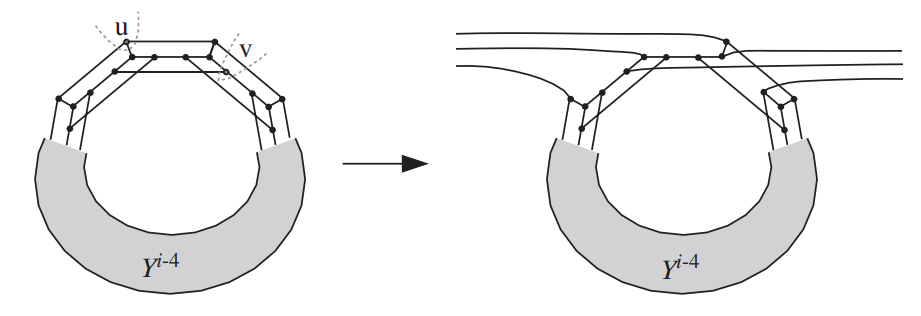
\includegraphics[width=0.6\textwidth]{images/create-Fi-from-Isaacs}
		\caption{\cite{Macajova2006} Construction of 6-pole $F^i$ from Isaacs snark $I_i$}
		\label{fig:construction-fi-from-isaacs}
	\end{figure}

	\begin{figure}
		\centering
		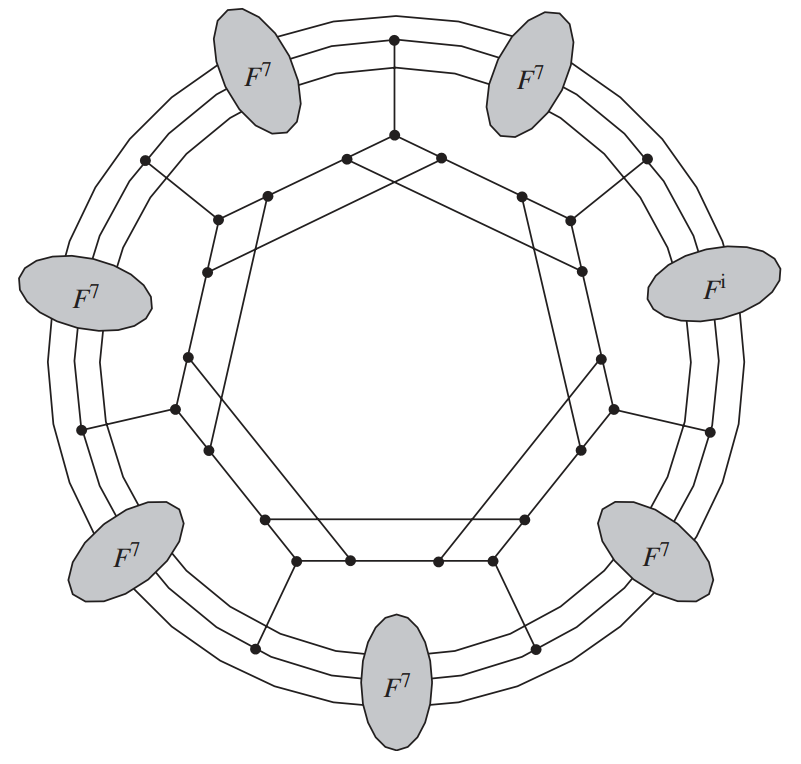
\includegraphics[width=0.5\textwidth]{images/snark-Gi-from-Isaacs}
		\caption{\cite{Macajova2006} Cyclically 6-connected graph $G_{1,i}$}
		\label{fig:cyc-6-graph-Macajova}
	\end{figure}

	In 2006, Máčajová and Škoviera presented the graph $G_{1,i}$ \cite{Macajova2006}, shown in \cref{fig:cyc-6-graph-Macajova}. This graph can be viewed as a junction of several 6-poles $F^i$ ($i\geq 7$), which are derived from Isaacs snarks \cite{Isaacs1975} by removing two vertices as illustrated in \cref{fig:construction-fi-from-isaacs}. Specifically, the construction uses six copies of $F^7$ and one $F^i$ with arbitrary $i\geq 7$, along with the structure in the middle. Even though the authors describe this graph as a result of a superposition, we will not dive deep into this theory and present the result as a result of partial junctions.
	
	The authors presented this graph as having cyclic connectivity equal to 6, however they have not provided a formal proof supporting this statement. In this example we prove this statement by utilizing our theoretical framework.
	
	\begin{figure}
		\centering
		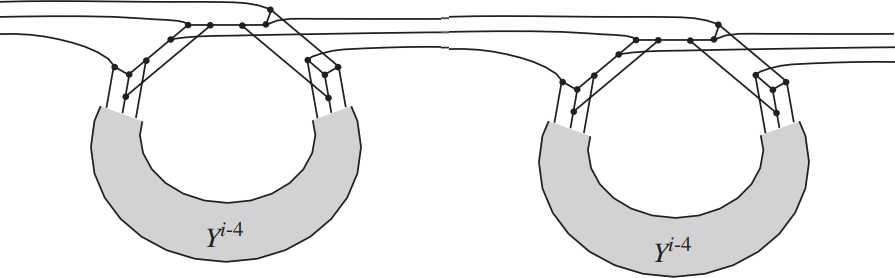
\includegraphics[width=0.6\textwidth]{images/Gi-first-partial-junction}
		\caption{Partial junction $F^i*F^j$}
		\label{fig:Gi-first-partial-junction}
	\end{figure}

	First observation is that each $F_i,~i\geq 7$ is potentially cyclically 6-connected. It has six semiedges, and we can verify that it does not contain a cyclic multipole with at most five semiedges. A helpful fact to verify this is that each Isaacs snark $I_i$ with $i\geq 7$ is cyclically 6-connected \cite{Mazak2022}. Secondly we see that the size of a smallest independent edge-cut in any $F_i$, $i\geq 7$ is two. However, when performing a partial junction between any two such multipoles ($F_i*F_j$ as shown in \cref{fig:Gi-first-partial-junction}), by denoting the semiedges used in the partial junction in $F_i$ and $F_j$ by $X_i$ and $X_j$ respectively, we can verify that $I_S(F_i,X_i)\geq 3$ and $I_S(F_j,X_j)\geq 3$. Thus by \cref{th:potentially-cyclically-connected-independent-semiedge-index} the result of the partial junction $F_i*F_j$ depicted in \cref{fig:Gi-first-partial-junction}  is potentially cyclically 6-connected. Let us denote the resulting multipole by $M_1$. We can verify that $M_1$ has no independent 2-edge-cut, thus $i(M_1)\geq 3$, which implies $I_S(M_1, X)\geq 3$ for any $X\subseteq S(M_1)$.
		
	\begin{figure}
		\centering
		\begin{subfigure}[b]{0.32\textwidth}
			\centering
			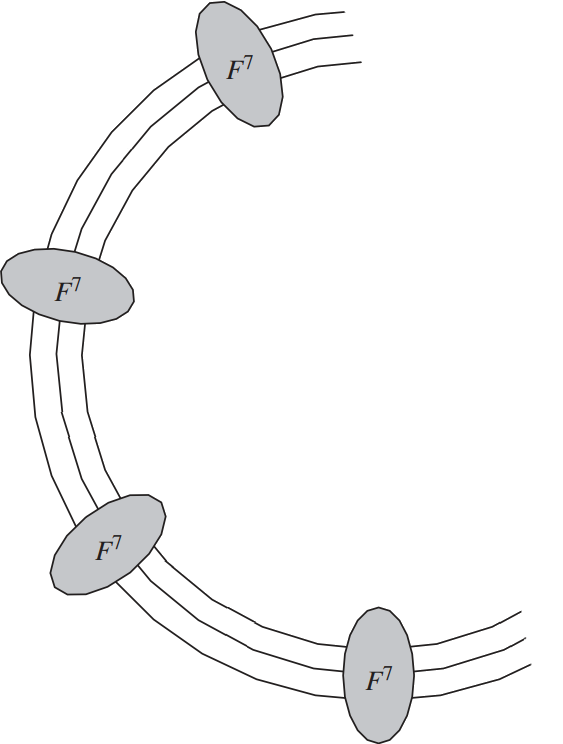
\includegraphics[height=5cm, width=\textwidth, keepaspectratio]{images/Gi-first-multipole}
			\caption{Multipole $N_1$}
			\label{fig:Gi-first-multipole}
		\end{subfigure}
		\hfill
		\begin{subfigure}[b]{0.32\textwidth}
			\centering
			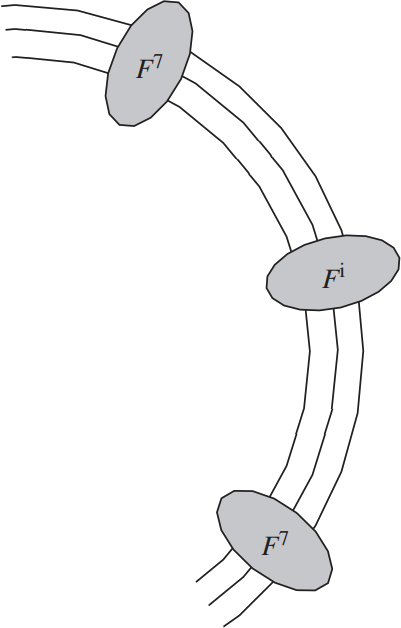
\includegraphics[height=5cm, width=\textwidth, keepaspectratio]{images/Gi-second-multipole}
			\caption{Multipole $N_2$}
			\label{fig:Gi-second-multipole}
		\end{subfigure}
		\hfill
		\begin{subfigure}[b]{0.32\textwidth}
			\centering
			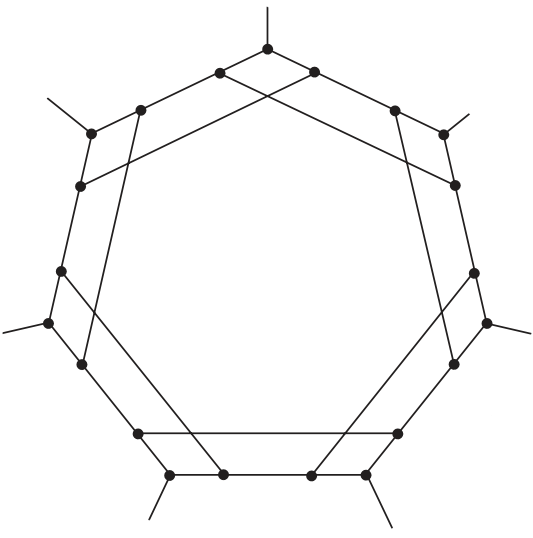
\includegraphics[height=5cm, width=\textwidth, keepaspectratio]{images/Gi-inner-multipole}
			\caption{Multipole $I$}
			\label{fig:Gi-inner-multipole}
		\end{subfigure}
		\caption{Multipoles used in building the graph $G_{1,i}$}
	\end{figure}

	Using this result, we can inductively construct multipole $N_1$, depicted in \cref{fig:Gi-first-multipole}, through multiple partial junctions with $F_i$. By \cref{th:potentially-cyclically-connected-independent-semiedge-index}, $N_1$ will be potentially cyclically 6-connected and it can be verified that it still holds that $i(N_1)\geq 3$. Similarly, we construct multipole $N_2$, depicted in \cref{fig:Gi-second-multipole}, with the same properties.
	
	\begin{figure}
		\centering
		\begin{subfigure}[b]{0.45\textwidth}
			\centering
			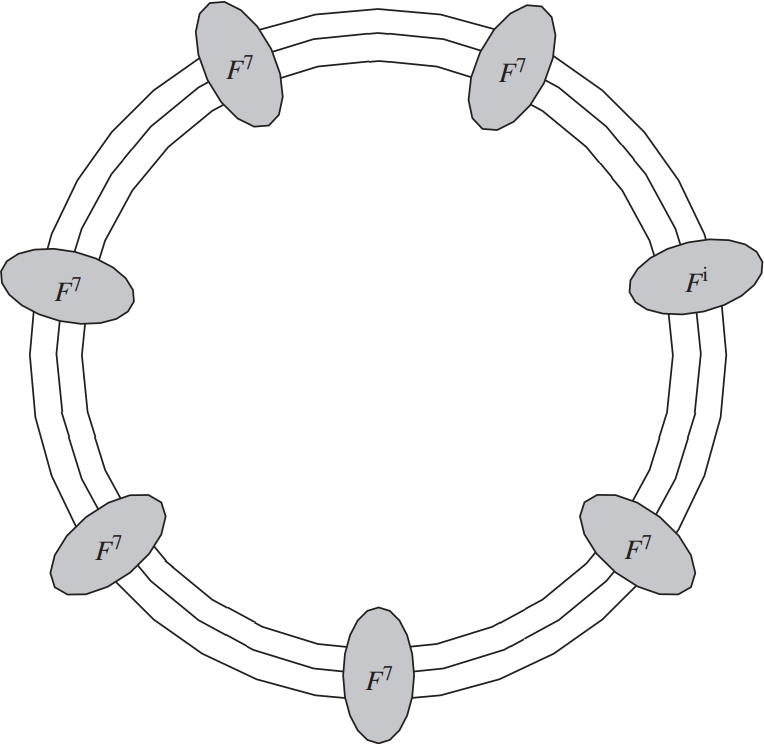
\includegraphics[width=\textwidth]{images/Gi-before-subdivision}
			\caption{Graph $N$}
			\label{fig:Gi-without-middle-before-subdivisions}
		\end{subfigure}
		\hfill
		\begin{subfigure}[b]{0.45\textwidth}
			\centering
			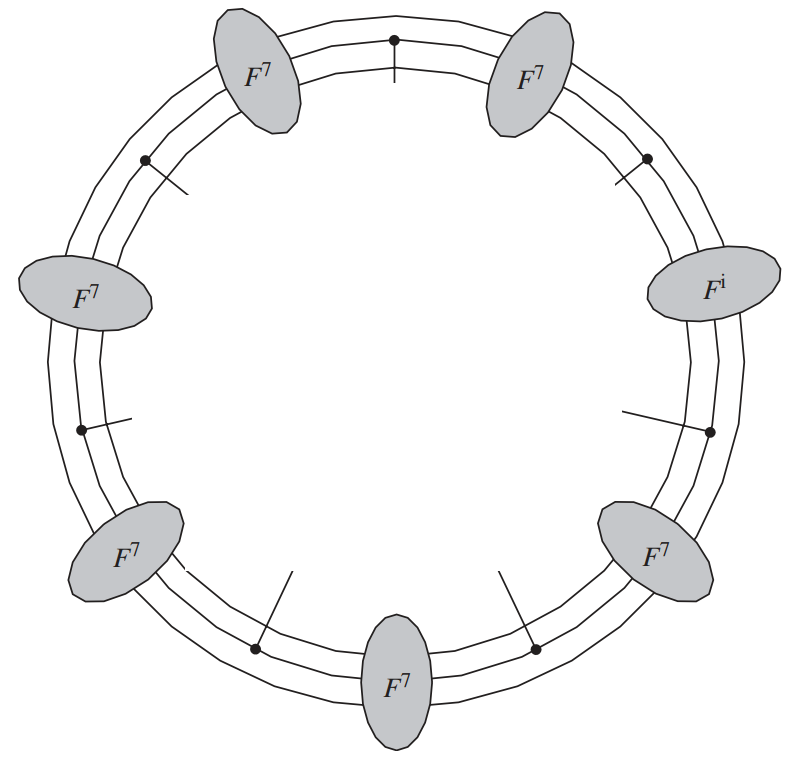
\includegraphics[width=\textwidth]{images/multipole-to-Gi-without-middle}
			\caption{Multipole $N'$}
			\label{fig:Gi-without-middle-after-subdivisions}
		\end{subfigure}
		\caption{$N$ before and after subdivisions}
	\end{figure}

	We then perform a junction $N_1*N_2$, resulting in graph $N$, as illustrated in \cref{fig:Gi-without-middle-before-subdivisions}. By \cref{th:cyclic-edge-connectivity-of-potentially-with-independent-cuts}, $N$ is cyclically 6-connected.
	
	Next, we perform seven edge subdivisions to obtain the multipole $N'$ depicted in \cref{fig:Gi-without-middle-after-subdivisions}. By \cref{th:subdivisions-potentially-cyclically-connected}, $N'$ is potentially cyclically 6-connected, and by \cref{lem:subdivisions-smallest-independent-cut}, $i(N')\geq 6$.
	
	Finally, let $I$ be the multipole shown in \cref{fig:Gi-inner-multipole}. We can verify that it is potentially cyclically 6-connected since it has 7 semiedges and contains no cyclic multipole with at most 5 semiedges. Therefore, since $i(N')\geq 6$, by \cref{th:cyclic-edge-connectivity-of-potentially-with-independent-cuts}, the final graph $G_{1,i}=N'*I$, depicted at the beginning in \cref{fig:cyc-6-graph-Macajova} is cyclically 6-connected.
\end{example}

Using our theoretical framework, we have formally proven that $G_{1,i}$ is indeed cyclically 6-connected, as claimed. However, this example has highlighted certain limitations in our framework. Firstly, we lack an efficient method for verifying that a multipole is potentially cyclically $k$-connected, even when we know the properties of the original graph from which the multipole was derived (in this case by removing a pair of vertices). Secondly, we had to manually verify the size of the smallest independent edge-cut in the multipoles, as the methods in our theoretical framework, specifically \cref{lem:size-of-minimal-independent-after-junction}, could not establish that this size was at least three. While these limitations required some manual verification steps, the majority of our proof relied on our theoretical framework. These challenges are explored in more detail in \cref{ch:problems-for-research}.

We now examine a similar construction from another article. While the proof follows a similar approach to the one presented above, some manual verification steps remain necessary.

\begin{example}
	\begin{figure}
		\centering
		\begin{subfigure}[b]{0.45\textwidth}
			\centering
			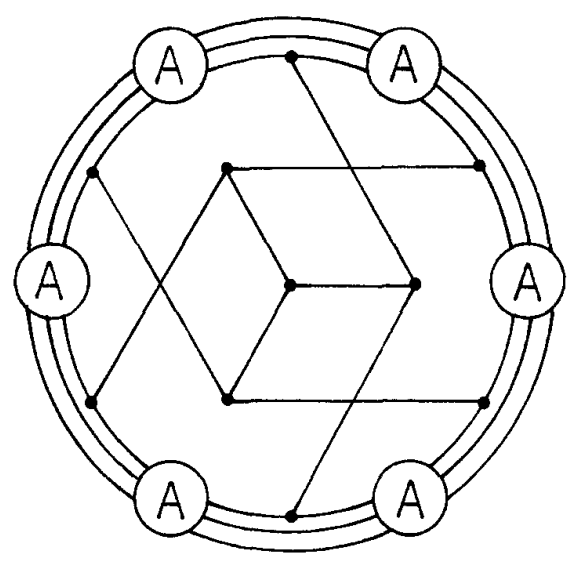
\includegraphics[width=\textwidth]{images/Kochol-article/Kochol-final-graph}
			\caption{Graph $G_{118}$}
			\label{fig:Kochol-final-graph-G118}
		\end{subfigure}
		\hfill
		\begin{subfigure}[b]{0.45\textwidth}
			\centering
			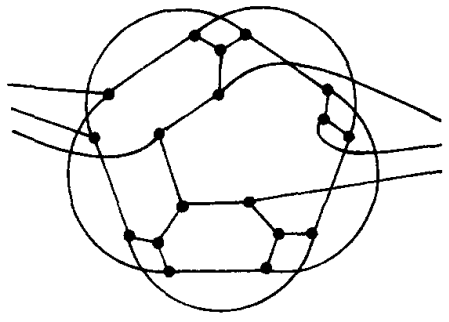
\includegraphics[width=\textwidth]{images/Kochol-article/Kochol-multipole-A}
			\caption{Multipole $A$}
			\label{fig:Kochol-multipole-A}
		\end{subfigure}
		\caption{\cite{Kochol1996} Graph $G_{118}$ built from multipoles $A$.}
	\end{figure}
	
	Consider the graph $G_{118}$ presented by Kochol in 1996 \cite{Kochol1996}, depicted in \cref{fig:Kochol-final-graph-G118}. This graph can be viewed as a junction of 6-poles $A$, created from Isaacs snark $I_5$ \cite{Isaacs1975} by removing two vertices, along with the construction in the middle of the cycle. The multipole $A$ is depicted in \cref{fig:Kochol-multipole-A}. Even though the author describes this graph as a result of a superposition, as before we will not dive deep into this theory and present the result as a result of partial junctions.
	
	The author presented this graph as having cyclic connectivity equal to 6, however without a formal proof. In this example we prove this statement by utilizing our theorems.
	
		\begin{figure}
		\centering
		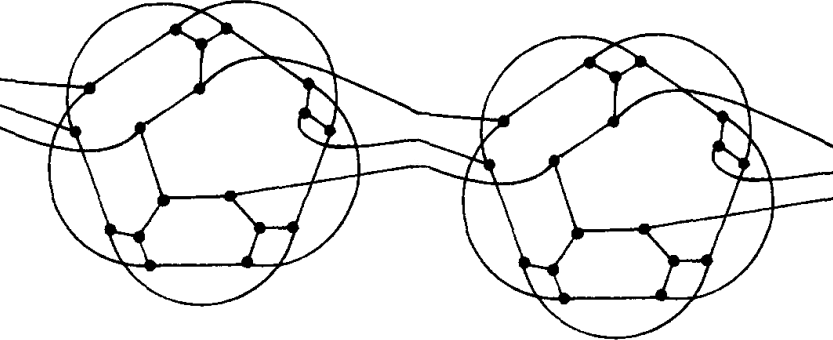
\includegraphics[width=0.6\textwidth]{images/Kochol-article/Kochol-multipoles-first-junction}
		\caption{Partial junction $A*A$}
		\label{fig:Kochol-first-partial-junction}
	\end{figure}
	
	First observation is that $A$ is potentially cyclically 6-connected. It has six semiedges, and we can verify that it does not contain a cyclic multipole with at most five semiedges. Secondly we see that the size of a smallest independent edge-cut in $A$ is two. However, when performing a partial junction between two copies of $A$ ($A*A$ as shown in \cref{fig:Kochol-first-partial-junction}), by denoting the semiedges used in the partial junction by $X_1$ and $X_2$ respectively, we can verify that $I_S(A,X_i)\geq 3$ for both $i\in\{1,2\}$. By \cref{th:potentially-cyclically-connected-independent-semiedge-index} the result of the partial junction $A*A$ depicted in \cref{fig:Kochol-first-partial-junction} is potentially cyclically 6-connected. Let us denote this construction by $M_1$. We can verify that $M_1$ has no independent 2-edge-cut, thus $i(M_1)\geq 3$, which implies $I_S(M_1, X)\geq 3$ for any $X\subseteq S(M_1)$.
	
	\begin{figure}
		\centering
		\begin{subfigure}[b]{0.45\textwidth}
			\centering
			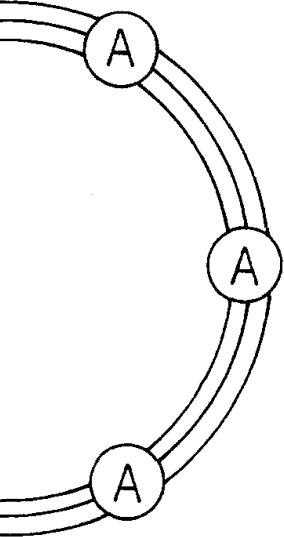
\includegraphics[height=5cm, width=\textwidth, keepaspectratio]{images/Kochol-article/Kochol-building-multipole}
			\caption{Multipole $N$}
			\label{fig:Kochol-first-multipole}
		\end{subfigure}
		\hfill
		\begin{subfigure}[b]{0.45\textwidth}
			\centering
			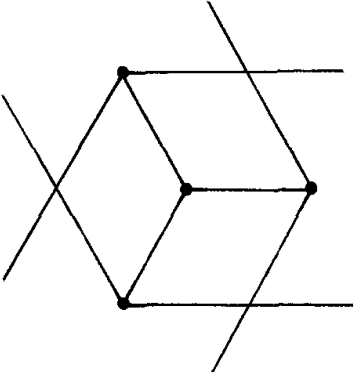
\includegraphics[height=5cm, width=\textwidth, keepaspectratio]{images/Kochol-article/Kochol-inner-multipole}
			\caption{Multipole $I$}
			\label{fig:Kochol-inner-multipole}
		\end{subfigure}
		\caption{Multipoles used in building the graph $G_{118}$}
	\end{figure}
	
	Using this result, we can inductively construct two copies of multipole $N$, depicted in \cref{fig:Kochol-first-multipole}, through multiple partial junctions with $A$. By \cref{th:potentially-cyclically-connected-independent-semiedge-index}, $N$ is potentially cyclically 6-connected and it can be verified that it still holds that $i(N)\geq 3$.
	
	\begin{figure}
		\centering
		\begin{subfigure}[b]{0.45\textwidth}
			\centering
			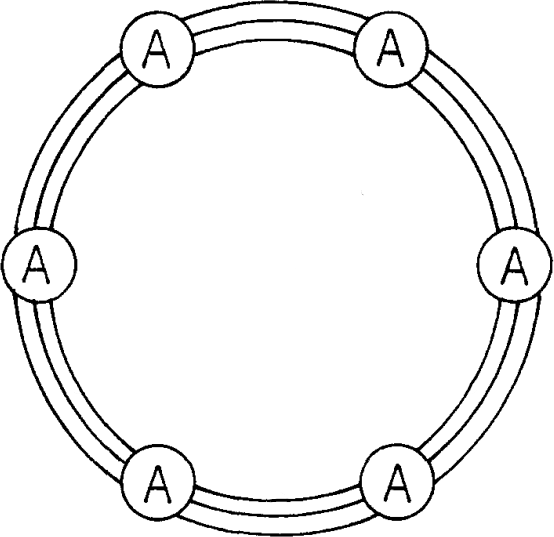
\includegraphics[width=\textwidth]{images/Kochol-article/Kochol-before-subdivisions}
			\caption{Graph $G$}
			\label{fig:Kochol-before-subdivisions}
		\end{subfigure}
		\hfill
		\begin{subfigure}[b]{0.45\textwidth}
			\centering
			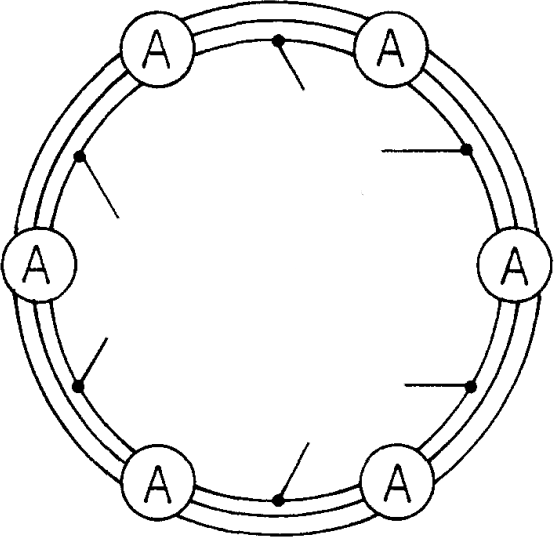
\includegraphics[width=\textwidth]{images/Kochol-article/Kochol-after-subdivisions}
			\caption{Multipole $G'$}
			\label{fig:Kochol-after-subdivisions}
		\end{subfigure}
		\caption{$N$ before and after subdivisions}
	\end{figure}
	
	We then perform a junction $N*N$, resulting in graph $G$, as illustrated in \cref{fig:Kochol-before-subdivisions}. By \cref{th:cyclic-edge-connectivity-of-potentially-with-independent-cuts}, $G$ is cyclically 6-connected.
	
	Next, we perform six edge subdivisions to obtain the multipole $G'$ depicted in \cref{fig:Kochol-after-subdivisions}. By \cref{th:subdivisions-potentially-cyclically-connected}, $G'$ is potentially cyclically 6-connected, and by \cref{lem:subdivisions-smallest-independent-cut}, $i(G')\geq 6$.
	
	Finally, let $I$ be the multipole shown in \cref{fig:Kochol-inner-multipole}. We see that $i(I)=1$. However, since it is acyclic and has six semiedges, it is potentially cyclically 6-connected. Since $i(G')\geq 6$, by \cref{th:cyclic-edge-connectivity-of-potentially-with-independent-cuts}, the final graph $G_{118}=G'*I$, depicted at the beginning in \cref{fig:Kochol-final-graph-G118} is cyclically 6-connected.
\end{example}

\chapter{Cyclic part inflations}\label{ch:cyclic-part-inflations}

The concept of inflations was previously established in \cref{sec:inflations}, where we presented the necessary definitions and the main theorem. This construction is particularly interesting as it enables the transformation of a graph through an "inflation" process, yielding a larger graph whose cyclic edge-connectivity can be determined from specific properties of the original graph.

This chapter introduces a modification to the mentioned inflation construction. While inflations involve replacing each vertex with a cycle whose length corresponds to the vertex degree, we propose \textit{cyclic part inflations}, where vertices are substituted with cyclic $k$-parts, where $k$ represents the degree of the respective vertex.

The chapter begins with essential definitions that formalize this operation, followed by our first theorem, which extends and modifies \cref{th:inflations-cyclic-connectivity} mentioned in the chapter about inflations. Subsequently, we present a second theorem accompanied by an illustrative application. This latter theorem emerged during examining the example mentioned afterwards, when we have proved it specifically for that example, and then made it more abstract to fit a broader class of graphs.

Let $G$ be a graph obtained by a sequence of partial junctions between cyclic parts $P_1,\dots,P_n$. A set of vertices $V\subseteq V(G)$ \textit{corresponds} to a cyclic part $P$ if $V=V(P)$.

We now formally define the concept of cyclic part inflations. Note that the graph from which we create inflations is arbitrary, thus does not have to be cubic.

\begin{definition}
	\label{def:cyclic-part-inflation}
	Let $G$ be an arbitrary graph and let $H$ be a cubic graph resulting from performing partial junctions on cyclic parts $P=\{P_1,\cdots,P_n\}$. Let $V=\{V_1,\cdots, V_n\}$ be a partition of $V(H)$ such that for each $i$ from 1 to $n$ the set $V_i$ corresponds to the cyclic part $P_i$. Then $H$ is called a \textit{cyclic part inflation} of $G$ if the graph obtained from $H$ by contracting each set $V_i\in V$ into a single vertex is isomorphic to $G$. The set of all cyclic part inflations of $G$ is denoted by $I_P(G)$.
\end{definition}

Similarly if we have a vertex $v\in G$ and some cyclic part inflation $H\in I_P(G)$, we say that the vertex $v$ corresponds to the set of vertices $V\subseteq V(H)$, if $V$ corresponds to some cyclic part $P$ in $H$ and by contracting we get the vertex $v$.

For inflations it has been proved, that in specific cases if the original graph is $k$-connected, then each of its inflations is cyclically $k$-connected (\cref{th:inflations-cyclic-connectivity}). First observation about these cyclic part inflations is in the form of a lemma, and is basically saying, that cyclic edge-connectivity of the inflation is bounded from above by the edge-connectivity of the former graph.

\begin{lemma}
	Let $G$ be a nontrivial graph with $\lambda(G)=k$. Then for each $H\in I_P(G)$ it holds that $\zeta(H)\leq k$.
\end{lemma}

\begin{proof}
	Let $S$ be a smallest edge-cut in $G$ separating it into components $M_1$ and $M_2$, and $G'$ be a cyclic part inflation from $I_P(G)$. In $G'$ this edge-cut is cycle-separating, since there is at least one cycle in each component which arose after the cyclic part inflation, and is of size $k$, thus the size of a smallest cycle-separating cut in $G'$ must be at most $k$.
\end{proof}

We now prove our modified version of \cref{th:inflations-cyclic-connectivity}. Although the proof follows a similar structure to the original theorem, we have made several adjustments to accommodate arbitrary cyclic parts. It is worth noting that traditional inflations can be viewed as a special case of cyclic part inflations, since \cref{lem:each-cycle-cyclic-part} shows that all $k$-cycles are cyclic parts. This means our new theorem naturally extends to cover both traditional inflations as well as cyclic part inflations.

\begin{theorem}\label{th:cyclic-part-inflations}
	Let $k\geq 3$ and let $G$ be a $k$-connected graph with girth at least $k$. Then every  $H\in I_P(G)$ is cyclically $k$-edge-connected.
\end{theorem}

\begin{proof}
	Let $H\in I_P(G)$. For each vertex $v\in V(G)$, denote the unique cyclic part in $H$ corresponding to it by $P_v$. We say that a cycle $C$ in $H$ is \textit{traversal} if there are two distinct vertices $v_1,v_2$ in $G$ with $V(P_v)\cap V(C)\neq \emptyset$ for both $v\in\{v_1,v_2\}$, so it goes through two unique cyclic parts in $H$. Otherwise we say that $C$ is \textit{non-traversal}, meaning $C\subseteq P_v$ for some $v\in V(G)$.
	
	Suppose by contradiction, that $H$ is not cyclically $k$-edge-connected. Then $H$ has a cycle-separating edge-cut $S$ with $|S|\leq k-1$ such that $H-S$ has precisely two cyclic components $D_1$ and $D_2$.
	
	Let $D_i^G$ be the subgraph of $G$ induced by the vertex set $$\{x\in V(G)~|~ V(P_x)\cap V(D_i)\neq \emptyset\},$$ so vertices from $G$, whose corresponding cyclic parts in $H$ have at least one vertex overlapping with the component $D_i$. Let us define sets $S_V$ and $S_E$ as
	\begin{align*}
		S_V &= \{x\in V(G) ~|~ E(P_x)\cap S\neq \emptyset\} \\
		S_E &= \{e\in S ~|~ \forall x\in V(G): e\notin E(P_x) \}.
	\end{align*}
	
	This means, that $S_V$ are vertices from $G$ whose corresponding cyclic parts contain at least one edge from $S$ and $S_E$ are edges from $S$ which are in no cyclic part, or in other words connect two vertices in $G$ and connect two cyclic parts in $H$. It can be seen that ${V(D_1^G)\cap V(D_2^G)=S_V}$, since the set contains vertices, whose corresponding cyclic parts contain edge from $S$, thus are split into the two components.
	
	Since $S_V$ contains vertices and $S_E$ contains edges, these sets are naturally disjoint, leading to $|S_V\cup S_E|=|S_V|+|S_E|$. To prove that $|S_V\cup S_E|\leq |S|$, we will show that each element in $S_V\cup S_E$ corresponds to at least one unique representative in $S$. This correspondence can be understood as an injective function from $S_V\cup S_E$ to $S$, which we demonstrate through two cases for an element $x$ from $S_V\cup S_E$:
	\begin{enumerate}
		\item When $x$ is a vertex ($x\in S_V$): The representatives in $S$ are the edges in $P_x$ that appear in the edge-cut $S$. These representatives cannot overlap with those of any other element from $S_V\cup S_E$. For a different vertex $y\in S_V$, its edges in $P_y$ will be distinct from those in $P_x$. Similarly, for edges in $S_E$, the representatives remain distinct, as explained in the next case.
		\item When $x$ is an edge ($x\in S_E$): These are edges from $S$ that don't belong to any cyclic part. For clarity, let's denote such edge as $e$. Its representative in $S$ is simply the edge itself. Again, this representative cannot overlap with those of other elements in $S_V\cup S_E$: for vertices in $S_V$, their representatives are edges from their respective $P_y$, which don't include $e$, and for other edges in $S_E$, their representatives are edges distinct from $e$.
	\end{enumerate} 
	
	This means, that $|S_V\cup S_E|\leq |S|$, which means after putting everything together that $$|S_V|+|S_E|=|S_V\cup S_E|\leq |S|\leq k-1.$$
	
	Suppose that $V(D_i^G)-S_V\neq\emptyset$ for each $i\in \{1,2\}$, meaning there is a whole cyclic part in both $D_1$ and $D_2$. We peove that by removing vertices $S_V$ and edges $S_E$ from $G$ we obtain a disconnected graph. Let $P_1$ and $P_2$ be the whole cyclic parts in $D_1$ and $D_2$ respectively. Let $v_1$ and $v_2$ be their corresponding vertices in $G$ respectively. Suppose there is a path between $v_1$ and $v_2$ in $G-S_v^G-S_E$. This path goes through edges not in $S_E$ and vertices not in $S_V$. This would hovever mean that there is path in $H-S$ between a vertex in $P_1$ and a vertex in $P_2$: it would go through the uncut edges not in $S_E$ and cyclic parts whose corresponding vertices in $G$ are not in $S_V$, leading to a contradiction.
	
	Thus $G-S_v^G-S_E$ has two components $F_1^G$ and $F_2^G$. The number of vertex disjoint paths from a vertex of $F_1^G$ to a vertex of $F_2^G$ in $G$ is at most $|S_V|+|S_E|\leq k-1$, since each path must go through either through a vertex in $S_V$, or edge in $S_E$, which contradicts by Menger's Theorem that $G$ is $k$-connected.
	
	Therefore we may assume without loss of generality that $V(D_1^G)-S_V=\emptyset$, meaning there is no whole cyclic part in $D_1$.
	
	Another thing to note is that in this case the component $D_2$ must contain at least one unsplit cyclic part, or in other words $V(D_2^G)-S_V\neq\emptyset$. Suppose that $V(D_2^G)-S_V=\emptyset$, which would mean that each cyclic part has been split by $S$. However $G$ is $k$-connected, thus $|V(G)|>k$ and since $S$ contains an edge from each of the cyclic parts it must hold that $|S|\geq |V(G)|>k$ which contradicts that $|S|\leq k-1$.
	
	\begin{figure}
		\centering
		\begin{tikzpicture}[every node/.style={circle, draw, fill=white, minimum size=15pt},scale=1.3]
			\node[minimum width=3cm, thick] (A) at (0,0) {};
			
			\draw[thick] ($(A.west) + (0.2,0.6)$) -- ++(-1.15,0);
			\draw[thick] ($(A.west) + (0.05,0.2)$) -- ++(-1,0);
			\draw[thick] ($(A.west) + (0.05,-0.2)$) -- ++(-1,0);
			\draw[thick] ($(A.west) + (0.2,-0.6)$) -- ++(-1.15,0);
			
			\draw[thick] ($(A.east) + (-0.2,0.6)$) -- ++(1.15,0);
			\draw[thick] ($(A.east) + (-0.05,0.2)$) -- ++(1,0);
			\draw[thick] ($(A.east) + (-0.05,-0.2)$) -- ++(1,0);
			\draw[thick] ($(A.east) + (-0.2,-0.6)$) -- ++(1.15,0);
			
			\draw[dashed, thick] (0,1.7) -- (0,-1.7);
			\node[draw=none] at (0,2) {$S_P$}; 
			\node[draw=none] at (-2.8,0) {$E_1$}; 
			\node[draw=none] at (2.8,0) {$E_2$}; 
			
			\node[draw=none] at (-0.45,-0.65) {$V_1$}; 
			\node[draw=none] at (0.45,-0.65) {$V_2$}; 
			\node at (-0.55,0) {$C_1$}; 
		\end{tikzpicture}
		\caption{Cyclic part $P_v$}
		\label{fig:P_v-cyclic-part}
	\end{figure}
	
	By assumption $D_1$ contains a cycle, say $C_1$. Suppose that this cycle is non-traversal, thus $C_1\subseteq P_v$ for some $v\in V(G)$. It must hold that $v\in S_V$, since there is no unsplit cyclic part in $D_1$, meaning $P_v$ has been split by $S$. Let $V_1$ and $V_2$ be the sets of vertices from $P_v$ in $D_1$ and $D_2$ respectively. Let $S_P=S\cap E(P_v)$ and let $E_1$ and $E_2$ be the sets of semiedges in $P_v$, which have one edge end incident with a vertex in $V_1$ or $V_2$ respectively as visible in \cref{fig:P_v-cyclic-part}. It is evident that if $P_v$ is a cyclic $m$-part, $|E_1|+|E_2|=m$. If $|S_P|<|E_2|$, the cut $S_P$ in $P_v$ would yield a cyclic $n$-pole, with $n=|E_1|+|S_P|<|E_1|+|E_2|=m$ leading to a contradiction by \cref{lem:cyclic-part-no-small-cyclic-l-pole}. Thus $|E_2|\leq |S_P|$.
	
	Let us denote the sets of edges in $H$ which were created by the junction of semiedges in $E_1$ or $E_2$ with some other semiedges as $L_1$ and $L_2$ respectively. It is evident that $|L_i|=|E_i|$ for both $i\in\{1,2\}$. We can now create an edge-cut $S'=(S-S_P)\cup L_2$. This cut is cycle separating as both components now contain a whole cyclic part and $|S'|\leq |S|\leq k-1$. Since both components now contain a whole cyclic part, this contradicts the assumption that $G$ is $k$-connected, as it was proved before.
	
	This means, that $C_1$ must be traversal. Thus $C_1$ corresponds to a closed trail in $D_1^G$, say $C_1^G$. Since the girth of $G$ is at least $k$ and every closed trail contains a cycle, we have $|V(C_1^G)|\geq k$. It holds that $V(C_1^G)\subseteq V(D_1^G)$ and because each cyclic part in $D_1$ has been cut we have $V(C_1^G)\subseteq V(D_1^G)\subseteq S_V$. From $|S_V|+|S_E|\leq k-1$ it leads to a contradiction with the fact that $|V(C_1^G)|\geq k$ since $V(C_1^G)\subseteq V(D_1^G)\subseteq S_V$ and $|S_V|\leq k-1$.
\end{proof}

Although this theorem is useful for determining cyclic edge-connectivity when performing junctions of multiple cyclic parts, it has some limitations regarding how these junctions can be performed. For instance, we cannot apply this theorem to graphs where two cyclic parts are connected by multiple edges. This is because the original graph would then contain vertices connected by multiple edges, resulting in a girth of at most two -- less than the required minimum of three.

To overcome this limitation, we present a new theorem that removes the restriction of having at most one edge between pairs of semiedges. Instead, it requires a larger number of edges connecting pairs of cyclic parts.

\begin{theorem}\label{th:cyclic-part-inflation-kve}
	Let $G$ be an arbitrary graph on $v$ vertices, such that each pair of vertices is connected by at least $e$ edges and let $k$ be an integer greater than zero for which it holds that
	$$k\leq 2e(v-2).$$
	Let $H$ be a cyclic part inflation of $G$. If $\lambda(G)\geq k$ and for each used cyclic part $M$ it holds that $i(M)\geq \frac{k}{2}$, then $H$ is cyclically $k$-connected.
\end{theorem}

\begin{proof}
	We can write the conidition inequality equivalently as $v\geq \frac{k+4e}{2e}$.
	
	Suppose that $H$ is not cyclically $k$-connected, thus it contains an independent \mbox{edge-cut} $S$ of size $l<k$, such that $l$ is the minimal possible. Let us denote the two cyclic components yielded by this cut by $X$ and $G-X$. By only cutting $l$ edges from the former graph $G$ we do not obtain a disconnected graph since $\lambda(G)\geq k$, thus $S$ contains some edges from the cyclic parts. Let $M$ be a cyclic part containing edges from the cut. These edges disconnect $M$ since it is a minimal cut, if it would not disconnect $M$ we could leave these edges out and obtain a smaller cut, contradicting the assumption about $l$. Since the cut is independent it needs to contain at least $\frac{k}{2}$ edges from $M$.
	
	If $S$ contained edges from another cyclic part it would have size at least $2\frac{k}{2}=k$ leading to a contradiction with the assumption that $|S|<k$. Thus other edges in $S$ must be former edges from $G$.
	
	Note that $\delta(G)\geq k$, since $\delta(G)\geq \lambda(G)\geq k$. Other than the part of $M$, there must be some whole cyclic parts in $X$. Otherwise $X$ would be whole in $M$, contradicting that $M$ is a cyclic $m$-part for $m\geq k$ by \cref{lem:cyclic-part-no-small-cyclic-l-pole}.
	
	The maximum number of whole cyclic parts in $X$ must be $v-2$ though. If all $v-1$ whole cyclic parts were in $X$, then $H-X$ would be a cyclic $l$-pole in $M$ again leading to a contradiction.
	
	Let $n$ be the number of whole cyclic parts in $X$. To make the graph disconnected, we need to cut all edges from these cyclic parts to the other ones. Each is connected to another by at least $e$ edges, thus we need to cut at least $ne(v-n-1)$ edges. The number $(v-n-1)$ represents the cyclic parts not in $X$, and $ne$ since each cyclic part in $X$ needs to be cut from the ones in $H-X$ by at least $e$ edges. We prove that $ne(v-n-1)\geq\frac{k}{2}$ for each $n$ from $1$ to $v-2$.
	
	By equivalent editing the inequality we get
	\begin{align*}
		ne(v-n-1)&\geq\frac{k}{2} \\
		2ne(v-n-1)&\geq k \\
		-2en^2+2nev-2ne&\geq k \\
		-2en^2+2ne(v-1)-k&\geq 0.
	\end{align*}
	This is a quadratic function in $n$, and since the coefficient of $n^2$ is negative, the parabola opens downward. Therefore, we only need to verify that the inequality holds at both endpoint values.
	
	For $n=1$ we get $e(v-2)\geq \frac{k}{2}$. For $n=v-2$ we get $(v-2)e(v-(v-2)-1)\geq\frac{k}{2}$, which can be simplified to the form $(v-2)e\geq\frac{k}{2}$, which is the same inequality as for $n=1$. thus we need to prove just this one.
	
	We know that $v\geq \frac{k+4e}{2e}$, thus it holds that $e(v-2)\geq e(\frac{k+4e}{2e}-2)$ and the sufficient proof will be $e(\frac{k+4e}{2e}-2)\geq \frac{k}{2}$.
	
	\begin{align*}
		e\left(\frac{k+4e}{2e}-2\right)&\geq \frac{k}{2} \\
		2e\left(\frac{k+4e}{2e}-2\right)&\geq k \\
		k+4e-4e&\geq k \\
		k&\geq k
	\end{align*}
	which is true thus the inequality holds. This means that each independent cut must contain at least $\frac{k}{2}$ edges in some cyclic part and at least $\frac{k}{2}$ edges not in any cyclic part, which is in total at least $k$, leading to a contradiction that the size of the cut $S$ is less than $k$.
\end{proof}

This theorem holds even for large $v,e$ and small $k$, which might lead to an understanding that this is not really an interesting theorem. For example if $v=10,e=3$ and $k=6$, we have a graph $H$ with 10 vertices, each pair of them connected by at least three edges, fulfilling the conditions from this theorem and we prove that a cyclic part inflation of $H$ is cyclically 6-connected. However the minimal degree of $H$ is at least $(v-1)e$, since each vertex is connected to each other by at least $e$ edges, specifically in this case it is equal to 27. Thus the cyclic part inflation of $H$ results from a sequence of partial junction of such cyclic parts, that the smallest possible $k$ for which it can be a cyclic $k$-part is 27. And proving if a junction of multiple cyclic 27-parts is cyclically 6-connected might not seem that interesting.

Ideally we would need for the minimal degree of $H$ to be equal to $k$. That way the cyclic part inflation will be a junction of multiple cyclic parts, such that at least one of them will be a cyclic $k$-part. That way we can prove that the cyclic $k$-part used in the cyclic part inflation will stay a cyclic $k$-part even in the whole graph, or in other words the cyclic edge-connectivity will be equal to $k$.

Ideally for this we would need for $k,v,e$ to fulfill a second inequality where ${k\geq (v-1)e}$, or equivalently $\frac{k+e}{e}\geq v$. This way we know that the minimum possible degree for such $v$ and $e$ will be at most $k$, thus by adding some edges to the vertices with lower degree we could obtain a graph with minimum degree equal to $k$ still satisfying the inequality from \cref{th:cyclic-part-inflation-kve}. If the minimum degree was less than $k$, it would not satisfy the condition of being $k$-edge-connected, thus edges need to be added for this condition to be satisfied.

We prove that for each $k$ such graph with minimal degree equal to $k$ and fulfilling the conditions of \cref{th:cyclic-part-inflation-kve} exists by proving the following lemmas.

\begin{lemma}
	For each integer $k\geq 2$, there exist integers $e$ and $v$ satisfying
	
	$$\dfrac{k+e}{e}\geq v\geq \dfrac{k+4e}{2e}.$$
\end{lemma}

\begin{proof}
	Let $e=1$ and $v=k+1$. Substituting these values into the original inequality yields
	$$k+1\geq k+1\geq \dfrac{k+4}{2}.$$
	The left inequality is immediately satisfied by equality. For the right inequality, we proceed with the following equivalent transformations:
	\begin{align*}
		k+1&\geq \dfrac{k+4}{2} \\
		2k+2&\geq k+4 \\
		k+2&\geq 4 \\
		k&\geq 2
	\end{align*}
	Since this final inequality aligns with our initial assumption that $k\geq 2$, we have demonstrated the existence of suitable values for $e$ and $v$ that satisfy the required inequalities.
\end{proof}

This demonstrates that for any given $k$, we can find values $v$ and $e$ such that there exists a graph $G$ with $v$ vertices where each pair of vertices is connected by at least $e$ edges, and the minimum degree equal to $k$. Furthermore, by \cref{th:cyclic-part-inflation-kve}, any cyclic part inflation of $G$ will be cyclically $k$-connected if we use cyclic parts whose smallest independent edge-cuts have size at least $\frac{k}{2}$.

However as previously noted, the primary advantage of \cref{th:cyclic-part-inflation-kve} over \cref{th:cyclic-part-inflations} is its ability to allow multiple edges between pairs of vertices in the former graph. While our previous proof used $e=1$, we now extend this result by proving the following lemma that adds the condition for $e\geq 2$.

\begin{lemma}
	For each integer $k\geq 4, k\neq 5$, there exist integers $e\geq 2$ and $v$ satisfying
	$$\dfrac{k+e}{e}\geq v\geq \dfrac{k+4e}{2e}.$$
\end{lemma}

\begin{proof}
	We prove this result by considering even and odd values of $k$ separately.
	\begin{itemize}
		\item For even $k$, let $e=2$ and $v=\frac{k+2}{2}$. This yields
		$$\dfrac{k+2}{2}\geq \dfrac{k+2}{2}\geq \dfrac{k+8}{4}$$
		The left inequality holds by equality. For the right inequality, we obtain by equivalent transformations:
		\begin{align*}
			\dfrac{k+2}{2}&\geq \dfrac{k+8}{4} \\
			2k+4&\geq k+8 \\
			k+4&\geq 8 \\
			k&\geq 4
		\end{align*}
		This inequality is satisfied for all even $k\geq 4$.
		
		\item For odd $k$, let $e=2$ and $v=\frac{k+1}{2}$. This gives us
		$$\dfrac{k+2}{2}\geq \dfrac{k+1}{2}\geq \dfrac{k+8}{4}$$
		The left inequality is clearly satisfied. For the right inequality:
		\begin{align*}
			\dfrac{k+1}{2}&\geq \dfrac{k+8}{4} \\
			2k+2&\geq k+8 \\
			k+2&\geq 8 \\
			k&\geq 6
		\end{align*}
		This holds for all odd $k\geq 7$, thus covering all odd values $k\geq 4$ except 5.
	\end{itemize}
\end{proof}

These lemmas demonstrate that \cref{th:cyclic-part-inflation-kve} is not limited to the example in the following section, but applies to infinitely many graphs. While we proved it only for $e\leq 2$, the theorem holds for any graph satisfying the inequality and the other conditions.

Now we present specific examples that illustrate both theorems about cyclic part inflations.

\section{Examples}

We now proceed to demonstrate practical applications of the theorems presented in this chapter through several illustrative examples. Let us begin with an example that showcases the application of \cref{th:cyclic-part-inflation-kve}.

\begin{example}
	\begin{figure}
		\centering
		\begin{tikzpicture}[every node/.style={circle, draw, fill=black, minimum size=10pt, inner sep=0pt}]
			% Define vertices
			\node[label=left:$c_1$] (A) at (0,0) {};
			\node[label=right:$c_2$] (B) at (4,0) {};
			\node[label=above:$c_3$] (C) at (2,3.464) {};
			\node[label=right:$c_4$] (M) at (2,1.155) {};
			
			% Draw curved edges between vertices
			% Each pair has two edges, one bent left and one right
			
			% Edges between A and B
			\draw[bend left=5] (A) to (B);
			\draw[bend right=5] (A) to (B);
			
			% Edges between B and C
			\draw[bend left=5] (B) to (C);
			\draw[bend right=5] (B) to (C);
			
			% Edges between C and A
			\draw[bend left=5] (C) to (A);
			\draw[bend right=5] (C) to (A);
			
			% Edges between M and A
			\draw[bend left=5] (M) to (A);
			\draw[bend right=5] (M) to (A);
			
			% Edges between M and B
			\draw[bend left=5] (M) to (B);
			\draw[bend right=5] (M) to (B);
			
			% Edges between M and C
			\draw[bend left=5] (M) to (C);
			\draw[bend right=5] (M) to (C);
		\end{tikzpicture}
		\caption{Graph $G$ for creating cyclically 6-connected graphs}
		\label{fig:4-6-poles-before}
	\end{figure}

	\begin{figure}
		\centering
		\begin{tikzpicture}[every node/.style={circle, draw, fill=white, minimum size=15pt}]
			% Define vertices
			\node (A) at (0,0) {$C_1$};
			\node (B) at (4,0) {$C_2$};
			\node (C) at (2,3.464) {$C_3$};
			\node (M) at (2,1.155) {$C_4$};
			
			% Draw parallel straight edges between vertices
			
			% Edges between A and B
			\draw (A.10) -- (B.170);
			\draw (A.-10) -- (B.-170);
			
			% Edges between B and C
			\draw (B.120) -- (C.-40);
			\draw (B.140) -- (C.-60);
			
			% Edges between C and A
			\draw (C.240) -- (A.40);
			\draw (C.220) -- (A.60);
			
			% Edges between M and A
			\draw (M.220) -- (A.15);
			\draw (M.200) -- (A.35);
			
			% Edges between M and B
			\draw (M.-40) -- (B.165);
			\draw (M.-20) -- (B.145);
			
			% Edges between M and C
			\draw (M.100) -- (C.-100);
			\draw (M.80) -- (C.-80);
			
		\end{tikzpicture}
		\caption{Cyclically 6-edge-connected cyclic part inflation}
		\label{fig:4-6-poles-inflation}
	\end{figure}

	Let $G$ be a graph from \cref{fig:4-6-poles-before} and let $C_1,C_2,C_3,C_4$ be cyclic 6-parts, not necessarily distinct, such that $i(C_j)\geq 3$ for each $j\in\{1,2,3,4\}$. Let $H$ be a cyclic part inflation of $G$, such that each cyclic part $C_i$ corresponds to the vertex $c_i$ in $G$ for each $i\in\{1,2,3,4\}$, as visible in \cref{fig:4-6-poles-inflation}.
	
	Since the number of vertices ($v$) is four, each pair of vertices is connected by $2$ edges ($e$), we can choose $k=6$ and the inequality 
	$$k\leq 2e(v-2)$$
	will hold, specifically $6\leq 4\cdot 2$. It is evident that $\lambda(G)=6$ and the condition of the sizes of minimal independent edge-cuts in each cyclic part is fulfilled. This means that by \cref{th:cyclic-part-inflation-kve} the graph $H$ is cyclically 6-connected. By cutting out just one of the cyclic parts we obtain a cycle-separating edge-cut of size 6, thus $\zeta(H)=6$.
	
	This example emerged from a specific challenge encountered during the development of this thesis, specifically when investigating the necessary conditions for a graph $H$ to achieve a cyclic edge-connectivity equal to 6.
\end{example}

Now we present an example showcasing the use of \cref{th:cyclic-part-inflations}.

\begin{example}\label{ex:cyclic-part-inflations-first-theorem}
	\begin{figure}
		\centering
		\begin{tikzpicture}[
			vertex/.style={circle, draw, fill=black, minimum size=10pt, inner sep=0pt},
			]
			
			% Place vertices in a circle with labels
			\foreach \i [count=\n from 1] in {90,45,0,-45,-90,-135,180,135} {
				\node[vertex] (v\n) at (\i:3cm) {\n};
				\node[draw=none,fill=none] at (\i:3.8cm) {$v_{\n}$};
			}
			
			% Draw edges using foreach loops
			% Circular connections (to next vertex)
			\foreach \i in {1,...,7} {
				\draw (v\i) -- (v\the\numexpr\i+1\relax);
			}
			\draw (v8) -- (v1); % Complete the circle
			
			% Cross connections (+3 mod 8)
			\foreach \i in {1,...,8} {
				\pgfmathtruncatemacro{\nextnode}{Mod(\i+3,8)}
				\ifnum\nextnode=0 \pgfmathtruncatemacro{\nextnode}{8} \fi
				\draw (v\i) -- (v\nextnode);
			}
			
		\end{tikzpicture}
		\caption{Graph $G$ in \cref{ex:cyclic-part-inflations-first-theorem}}
		\label{fig:cyclic-part-inflations-ex-2-before}
	\end{figure}

	Let $G$ be the graph depicted in \cref{fig:cyclic-part-inflations-ex-2-before}. It can be verified that $\delta(G)=4$, $\kappa(G)=4$ and $g(G)=4$. This means that each cyclic part inflation $H$ of $G$ is cyclically 4-connected and since $\delta(G)=4$ it holds that $\zeta(H)=4$.
\end{example}


\chapter{Problems for further research}\label{ch:problems-for-research}

In this chapter, we present problems encountered during our research, including unresolved problems and questions that emerged later. Some of these issues arose from examples in \cref{subs:examples}, where we had to manually verify certain properties of multipoles, such as the size of a smallest independent edge-cut, when we could not apply our theoretical framework.

The first problem concerns the independent cut-semiedge index of a multipole created through partial junction. While we have developed a theoretical framework for establishing lower bounds on the size of smallest independent edge-cuts in multipoles formed by partial junctions, we lack similar results applicable for this index.

\begin{problem}
	Let $M=M_1*M_2$ be a multipole. Given the values $I_S(M_1,X_1)$ and $I_S(M_2,X_2)$, and considering another subset of semiedges $X\subseteq S(M)$, what is the lower bound of $I_S(M,X)$?
\end{problem}

This property presents unique challenges because it depends not only on the multipole itself but also on which semiedges will be used in future partial junctions. This makes it difficult to establish a lemma similar to \cref{lem:size-of-minimal-independent-after-junction}, as simply in independent edge-cuts we do not distinguish between semiedges that will remain and those used in the partial junction.

The following problem also comes from the exploring of the examples. Specifically, we obtained multipoles from Isaacs snarks by removing a pair of vertices. Despite knowing their cyclic edge-connectivity, we could not formally prove that multipoles obtained by removing these vertices were potentially cyclically $k$-connected without manual verification. A theoretical framework for deriving these properties from the original graph would be valuable.

\begin{problem}
	Let $G$ be a cyclically $k$-connected graph, with $i(G)\geq l$ for some $l,k$. For a multipole $M$ obtained from $G$ by removing vertices and/or severing edges, what conditions ensure that $M$ is potentially cyclically $k$-connected, and what determines the lower bound of $i(M)$?
\end{problem}

These conditions might be specific rather than general, for instance applying only to the removal of two vertices with a known distance between them.

Other than by a theoretical approach, it would be highly valuable to develop an algorithmic approach for determining whether a multipole is potentially cyclically $k$-connected.

\begin{problem}
	Develop an efficient algorithm that determines whether a given multipole $M$ is potentially cyclically $k$-connected for a given integer $k$.
\end{problem}

If $M$ is a graph, the problem is equivalent to the problem of determining whether $M$ is cyclically $k$-connected, thus the best approach is the algorithm by Dvořák et al. \cite{Dvorak2004}. A solution for multipoles might involve a modification of this algorithm to handle multipoles and search for cyclic multipoles with the smallest number of semiedges, or by performing a junction of the multipole on input with some other multipole, specific for this problem, and running the original algorithm.

Given the fundamental importance of the question whether a multipole is potentially cyclically $k$-connected in our work, developing an efficient method to determine this property would be particularly valuable.

Regarding inflations, we propose a modified approach where not every vertex needs to be inflated by a cyclic part -- some can remain as single vertices. It would be valuable to develop theorems for this modified approach.

\begin{problem}
	Consider a generalized form of cyclic part inflations where $H$ is a cyclic part inflation of $G$ if $H$ results from partial junctions of cyclic parts and single vertices, and $G$ can be obtained by contracting the sets of vertices corresponding to the used cyclic parts in $H$. Prove analogous results to \cref{th:cyclic-part-inflations,th:cyclic-part-inflation-kve} for this modified approach.
\end{problem}

Finally, while not formulated as a specific problem, it would be valuable to modify our theoretical framework to include isolated edges as well. Recall that these are edges which have both ends not incident with a vertex. Due to their unique behaviour during junctions, they were excluded from our framework. However, since isolated edges are commonly accepted in the literature, incorporating them would enhance the completeness and broader applicability of our framework.

\chapter*{Conclusion}
\addcontentsline{toc}{chapter}{Conclusion}
\markboth{Conclusion}{Conclusion}

In this thesis we have made several contributions to the study of cyclic edge-connectivity in cubic graphs, particularly focusing on constructions from smaller building blocks. Our work has extended existing theoretical frameworks and introduced new approaches for analyzing and constructing graphs with specific cyclic edge-connectivity.

Firstly, we have developed a theoretical framework for determining whether a cyclic multipole is a cyclic part without needing to find the original graph. The main result is formulated in \cref{th:alternative-definition-of-cyclic-part}, which establishes that a cyclic multipole is a cyclic part if and only if it does not contain a cyclic multipole with a small number of semiedges. This result provides a more direct method for identifying cyclic parts, eliminating the need for constructing the original graph from which the cyclic part could be obtained.

Secondly, we have established new conditions for junctions of multiple multipoles to achieve desired cyclic edge-connectivity. Our theoretical framework, particularly through \cref{th:connecting-potentially-cyclically-connected-with-number-of-resulting-semiedges,th:potentially-cyclically-connected-independent-semiedge-index,th:cyclic-edge-connectivity-of-potentially-with-independent-cuts}, provides specific conditions under which these constructions maintain cyclic edge-connectivity. These conditions primarily involve the sizes of smallest independent edge-cuts and the absence of cyclic multipoles with few semiedges. These results are particularly valuable as they apply to arbitrary values of the cyclic edge-connectivity, extending beyond the specific cases studied in previous research. In addition to these theorems, we have proven results regarding modifications of multipoles, for example by edge subdivisions.

Thirdly, we have introduced and analyzed the concept of cyclic part inflations, extending the traditional notion of inflations. Through \cref{th:cyclic-part-inflations,th:cyclic-part-inflation-kve}, we have established conditions under which these constructions preserve cyclic edge-connectivity, providing new methods for constructing cyclically $k$-connected graphs. This approach offers greater flexibility than traditional inflations, since it allows inflations of the graph not only with $k$-cycles, but arbitrary cyclic $k$-parts.

Our work has also demonstrated practical applications of these theoretical results through several examples, including verifying claims about the cyclic edge-connectivity of specific graphs made in previous publications without formal proofs. These examples not only validate our theoretical framework but also illustrate its practical utility in analyzing complex graph structures.

Finally, we present open problems that emerged during writing this thesis, suggesting potential directions for future research. These problems emerged primarily while verifying cyclic edge-connectivity in the mentioned examples, where our theoretical framework lacked methods for certain proofs, requiring manual verification instead.

% BIBLIOGRAPHY
\newpage
\thispagestyle{empty}

\bibliographystyle{plain}
\bibliography{references}

% APPENDICES
%\appendix
%\thesisappendices{}

\end{document}
